\documentclass[12pt,a4paper]{article}
\usepackage[utf8]{inputenc}
\usepackage[T1]{fontenc}
\usepackage{lmodern}
\usepackage[spanish,es-tabla,es-noquoting]{babel}
\usepackage[margin=2.5cm]{geometry}
\usepackage{graphicx,booktabs,longtable,tabularx,array,amsmath,amssymb}
\usepackage{float,subcaption,listings,xcolor,tikz}
\usetikzlibrary{arrows.meta,positioning,fit}
\usepackage{csquotes}
\usepackage[backend=biber,style=ieee,sorting=none]{biblatex}
\addbibresource{../entrega3/referenciasPFC.bib}
\usepackage{microtype}
\usepackage{hyperref}
\hypersetup{colorlinks=true,linkcolor=black,citecolor=black,urlcolor=blue,pdftitle={TiendaTech: documento acumulativo de cierre},pdfauthor={Equipo AGLS}}
\usepackage{xurl}
\setlength{\parindent}{0pt}
\setlength{\parskip}{0.6em}
\setlength{\emergencystretch}{3em}
\renewcommand{\arraystretch}{1.18}
\setcounter{tocdepth}{2}
\lstset{basicstyle=\ttfamily\footnotesize,breaklines=true,frame=single,columns=fullflexible,keepspaces=true,showstringspaces=false,captionpos=b}
\newcommand{\repo}{https://github.com/JoseLozanoMorales/TiendaTech}
\newcommand{\evidencia}[2]{\href{https://github.com/JoseLozanoMorales/TiendaTech/blob/62f0b15736926dffce5ead70acc55a89ec75f9ad/#1}{#2}}
\newcommand{\seccion}[1]{\section{#1}}
\begin{document}
\begin{titlepage}
\centering
\includegraphics[width=3.5cm]{UteqLogo.png}\par
\vspace{0.4cm}
{\Large Universidad Técnica Estatal de Quevedo\par}
{\large Aplicaciones Distribuidas -- Séptimo A\par}
\vspace{1cm}
{\Huge\bfseries TiendaTech\par}
\vspace{0.5cm}
{\Large Documento acumulativo E1--E4\par}
{\large Arquitectura, implementación y evaluación experimental\par}
\vspace{1cm}
{\large Proyecto Fin de Curso -- Paso 13\par}
\vspace{0.8cm}
\begin{tabular}{ll}
\toprule
Integrante & Rol asignado\\
\midrule
Jhinson Stalyn Aucatoma Celorio & Arquitecto\\
Jeremy Ruperto Gaibor Rodriguez & Desarrollador\\
Andy Paul Sanchez Pilaloa & Responsable de Calidad\\
José Alejandro Lozano Morales & Documentalista\\
\bottomrule
\end{tabular}
\vfill
Docente: Gleiston Cicerón Guerrero Ulloa\par
Período académico 2026\par
Corte documental: 1 de septiembre de 2026\par
\vspace{0.4cm}
{\large\textbf{FECHA PERMITIDO DE ÚLTIMO COMMIT:}\par}
{\large Viernes 4 de septiembre del 2026 hasta Hora: 20h00\par}
\url{https://github.com/JoseLozanoMorales/TiendaTech}\par
\end{titlepage}
\pagenumbering{roman}
\begingroup\setlength{\parskip}{0pt}\tableofcontents\endgroup
\clearpage\listoffigures
\clearpage\listoftables
\clearpage
\section*{Resumen}
\addcontentsline{toc}{section}{Resumen}
\textbf{Objetivo:} consolidar la evolución de TiendaTech y evaluar qué propiedades de su arquitectura distribuida quedan respaldadas por evidencia. \textbf{Método:} revisión del repositorio, mediciones de CockroachDB y Spark, y una campaña correctiva de 120 corridas mediante API Gateway, microservicios y CockroachDB, con dos estrategias, cuatro concurrencias y tres condiciones de fallo. \textbf{Resultados:} la matriz real contiene 208003 solicitudes y 49786 intentos de checkout, de los cuales 30275 fueron confirmados. Saga confirmó 63,4\,\% y 2PC 58,1\,\% en el agregado descriptivo; ninguna de las doce comparaciones de p95 resultó significativa con Bonferroni. El CSV no conserva historiales persistentes suficientes para acreditar invariantes. La evaluación ISO observó 3588/3588 sondeos exitosos durante una hora y un p95 de 610\,ms con 50 usuarios, superior al objetivo de 500\,ms. \textbf{Contribución:} una memoria trazable que separa implementación, medición y límites de inferencia. No se acredita una comparación reglas--RAG.

\textbf{Palabras clave:} sistemas distribuidos, coordinación, CockroachDB, Spark, calidad, reproducibilidad.
\clearpage
\section*{Abstract}
\addcontentsline{toc}{section}{Abstract}
\textbf{Objective:} to consolidate TiendaTech's evolution and determine which distributed-system properties are supported by evidence. \textbf{Method:} repository review, CockroachDB and Spark measurements, and a corrective campaign of 120 runs through the API Gateway, microservices and CockroachDB, covering two strategies, four concurrency levels and three fault conditions. \textbf{Results:} the real matrix contains 208,003 requests and 49,786 checkout attempts, of which 30,275 were confirmed. Saga confirmed 63.4\,\% and 2PC 58.1\,\% in the descriptive aggregate; none of the twelve p95 comparisons was significant after Bonferroni correction. The CSV does not retain persistent histories sufficient to establish invariants. The ISO assessment observed 3,588 successful probes out of 3,588 during one hour and a p95 of 610 ms with 50 users, above the 500 ms target. \textbf{Contribution:} a traceable report separating implementation, measurement and inference limits. A rules-versus-RAG comparison is not established.

\textbf{Keywords:} distributed systems, coordination, CockroachDB, Spark, quality, reproducibility.
\clearpage\pagenumbering{arabic}
\section{Introducción}
TiendaTech es un proyecto académico de comercio electrónico de componentes de computación. Integra clientes web y móvil, autenticación, catálogo, inventario, pedidos, ventas, compras a proveedores y un asistente de armado. El problema técnico consiste en conservar reglas de negocio cuando la información cruza procesos y se presentan reintentos, fallos de comunicación o indisponibilidad de datos. Una compra no debe confirmar un pago distinto del esperado, descontar inventario indebidamente ni permanecer en un estado parcial sin una política de recuperación.

La cuantificación disponible corresponde al entorno experimental, no a pérdidas comerciales de una empresa. El conjunto analítico histórico incluye 600\,000 pedidos y detalles, 10\,000 usuarios y 570\,000 filas tras el filtrado y unión. El ensayo de coordinación comprende 24 condiciones y cinco repeticiones por condición, con concurrencias nominales entre 50 y 400. Estos tamaños delimitan la evaluación: no se dispone de una línea base de incidentes ni de clientes reales que permita estimar impacto económico. La ausencia de esos datos no se reemplaza por cifras supuestas.

\subsection{Objetivos y alcance}
El objetivo general es documentar y evaluar una implementación distribuida reproducible, identificando sus garantías y límites. Los objetivos específicos son: describir las fronteras y decisiones arquitectónicas; relacionar consistencia, replicación y fallos con agregados del negocio; presentar mediciones de procesamiento y coordinación; contrastar calidad y revisión cruzada con evidencia; y responder las preguntas del banco experimental sin extrapolar más allá de su implementación.

La memoria acumula E1 (propuesta y decisiones), E2 (modelo y distribución de datos), E3 (integración y análisis) y E4 (refactor, seguridad, pruebas y evaluación). El nombre anterior del repositorio fue \texttt{PFC-AppsDistribuidas}; la denominación adoptada es TiendaTech. Esta aclaración conserva la interpretación de rutas y mensajes históricos. Las tres capturas de búsqueda del nombre se conservan en \path{docs/nombre/} desde el commit \texttt{ea0b4eb} del 26 de agosto. El buscador general y GitHub muestran coincidencias; SourceForge muestra cero resultados con el filtro Windows activo. Se documenta la búsqueda realizada, sin inferir exclusividad de la denominación. Su inventario y alcance están enlazados desde el README.

\subsection{Corte de evidencia y organización}
El corte documental integra las evidencias publicadas hasta el commit \texttt{62f0b15}, cuyo hash completo fijan los enlaces de evidencia. Incluye la campaña correctiva del 5 de septiembre, la evaluación ISO, las pruebas de CI, el panel Grafana y las trazas. Cada resultado conserva su procedencia y unidad experimental; el cierre de esta memoria no equivale a declarar aprobados los pasos técnicos que permanecen como deuda.

El texto avanza desde el estado del arte y el diseño hasta la implementación; define después el estudio, presenta resultados separados de su discusión y examina amenazas, calidad y revisión cruzada. Las conclusiones responden las preguntas experimentales; las reflexiones individuales, ética y declaraciones explicitan la responsabilidad del equipo. La bibliografía sigue estilo IEEE con Biber. Los identificadores de evidencias permiten localizar el dato original y diferenciarlo de su interpretación.
\subsection{Registro de cambios explícito frente a E1}
La tabla \ref{tab:cambios-e1} responde al ítem 2.1 del Paso 2: qué cambió respecto de la propuesta de E1 (\emph{TiendaTech: Propuesta y Análisis del Sistema Distribuido}, 27 de mayo de 2026) y por qué. No se trata de una lista de novedades técnicas sueltas, sino de la evolución de cada uno de los ocho compromisos de E1 hasta el corte documental integrado. Dos ítems se marcan explícitamente como parciales o pendientes: no se declara cumplido lo que todavía no tiene evidencia cerrada.

\begin{longtable}{>{\raggedright\arraybackslash}p{2.9cm}>{\raggedright\arraybackslash}p{5.5cm}>{\raggedright\arraybackslash}p{6.2cm}}
\caption{Registro de cambios frente a E1, ítems 2.1--2.8.}\label{tab:cambios-e1}\\
\toprule \textbf{Ítem} & \textbf{En E1} & \textbf{Qué cambió en E4 y por qué}\\\midrule
\endfirsthead
\toprule \textbf{Ítem} & \textbf{En E1} & \textbf{Qué cambió en E4 y por qué}\\\midrule
\endhead
\bottomrule
\endfoot

2.1 Problema cuantificado &
Cuantificación de mercado: facturación de e-commerce nacional (CECE, \textgreater 4\,000 M USD), hardware entre los tres sectores de mayor volumen. Motivación de negocio, no medida por el equipo. &
La Introducción sustituye la cifra de mercado por la cuantificación del propio entorno experimental: 600\,000 pedidos y detalles, 10\,000 usuarios, 570\,000 filas tras filtrado, 24 condiciones $\times$ 5 repeticiones del ensayo de coordinación. Se abandona una cita externa no verificable por el equipo y se sostiene el problema con datos que el propio proyecto puede respaldar: ``la ausencia de esos datos no se reemplaza por cifras supuestas''.\\

2.2 Justificación de arquitectura &
ADR-01 (E1): microservicios justificados por separación de responsabilidades y ``reducir el impacto de fallos'', consecuencias enunciadas como expectativa. &
``Despliegue y decisiones'' agrega la distinción explícita entre decisión y medición: ``no todas las consecuencias previstas en E1 se convirtieron en resultados medidos [...] demostrar que mejora latencia o disponibilidad requiere un experimento''. Cambio de una justificación cualitativa a una que declara qué de lo prometido en E1 sigue sin comprobarse.\\

2.3 Estado del arte $\geq$15 fuentes &
Matriz de 7 referencias (Cuadro 1 de E1), organizada en torno al problema de negocio (recomendación de catálogo, colisiones de compatibilidad, NLP/LLM). &
Cuatro subsecciones nuevas (consistencia y datos distribuidos, procesamiento paralelo, microservicios y clientes, pruebas y CI/CD) que inicialmente citaban 15 fuentes con DOI; la ampliación documental añade cinco específicas de 2PC y Saga. El estado del arte se reorienta de la motivación de negocio de E1 a la literatura que sostiene las decisiones técnicas realmente evaluadas en E2--E4 (CAP, relojes lógicos, Amdahl/Gustafson, CI/CD).\\

2.4 Diagramas C4 &
Figuras 1 (C4-L1) y 2 (C4-L2) insertadas como imagen, sin nivel de componentes (L3). &
``Contexto y contenedores'' y ``Componentes y capas'' reconstruyen L1 y L2 y agregan L3, con TikZ embebido y versionado como código fuente en vez de imagen suelta. La reconstrucción es necesaria porque la arquitectura real cambió (seis servicios Java, armado-ia en Python, gateway), no una actualización estética.\\

2.5 ADR &
Tres ADR fundacionales: 01 (microservicios), 02 (API Gateway), 03 (motor de compatibilidad). &
El corte referencia \texttt{docs/adr} con ADR-003 a ADR-012 (fragmentación temporal de pedidos, Raft, patrones de diseño, JWT, capas Python, recuperación de las tres decisiones de E1, fragmentación del catálogo) más dos registros móviles. De 3 decisiones fundacionales a un registro vivo de 12+ decisiones que cubre persistencia distribuida, seguridad y despliegue.\\

2.6 Posición CAP por agregado (datos del Paso 8) &
No existe tabla CAP; el ADR-01 solo menciona ``alta disponibilidad'' en abstracto, sin diferenciar por agregado. &
La tabla \ref{tab:cap} (``Consistencia por agregado'') formula una política CAP distinta para inventario, pedido/pago, usuarios, catálogo y analítica, cada una con su límite de evidencia declarado. \textbf{Actualización del 5 de septiembre:} la campaña correctiva de checkout produjo 30275 confirmaciones en 120 corridas contra el sistema desplegado, después de aprobar pilotos basales y una rampa de carga. Esa muestra permite describir disponibilidad y latencia del flujo, pero el CSV agregado no conserva historiales persistentes por operación ni ensaya una partición de red controlada; por ello todavía no valida la política CAP por agregado ni las cuatro invariantes de negocio.\\

2.7 Modelo de fallos de Cristian &
No existe modelo de fallos ni de sincronización de reloj en E1. &
``Modelo de fallos y orden'' cubre omisión, demora, caída de proceso y reintentos, y formaliza el \emph{orden} causal con relojes lógicos de Lamport (ecuación \ref{eq:lamport}). \textbf{Brecha real, no resuelta:} el ítem pide el algoritmo de Cristian (sincronización de reloj físico mediante intercambio de mensajes con un servidor de tiempo); el documento no lo menciona ni lo implementa. Lamport resuelve un problema relacionado pero distinto (orden lógico, no sincronización de reloj físico); no debe declararse cumplido este punto sin trabajo adicional.\\

2.8 Métricas y plan de validación &
Cuadro 2 de E1: 6 métricas ISO/IEC 25010 con umbral objetivo, sin plan de medición (sin repeticiones, descartes ni tratamiento estadístico). &
``Diseño del estudio'' agrega 5 preguntas operativas, la tabla \ref{tab:protocolo} que compara explícitamente lo pedido por la guía frente a lo realmente ejecutado (declarando discrepancias, p.\,ej.\ retardo de 0,05\,s frente a 5\,s pedidos), variables con oráculo de invariantes y análisis estadístico con bootstrap, Wilson, Mann--Whitney y tamaño de efecto $\widehat A_{12}$. De un cuadro de métricas objetivo sin plan, a un protocolo ejecutado y confrontado honestamente contra lo prometido.\\

\end{longtable}

\subsection{Registro de cambios por entrega}
La tabla \ref{tab:cambios-entregas} hace explícita la recuperación acumulativa solicitada en C1. Las bases históricas son \path{docs/entrega1/entrega1.pdf}, \path{docs/entrega2/entrega2.pdf} y \path{docs/entrega3/PFC3.tex}. La entrega de origen identifica el contenido recuperado; no significa que todos sus cambios se hayan realizado durante esa entrega. Los commits enlazados registran correcciones posteriores integradas en E4. Las reservas describen lo que todavía no queda demostrado.

{\small\setlength{\tabcolsep}{4pt}
\begin{longtable}{>{\raggedright\arraybackslash}p{1.1cm}>{\raggedright\arraybackslash}p{3.4cm}>{\raggedright\arraybackslash}p{6.3cm}>{\raggedright\arraybackslash}p{3.6cm}}
\caption{Registro explícito de recuperación y correcciones E1--E4.}\label{tab:cambios-entregas}\\
\toprule Origen & Base o aspecto revisado & Cambio integrado y límite & Evidencia histórica\\\midrule\endfirsthead
\toprule Origen & Base o aspecto revisado & Cambio integrado y límite & Evidencia histórica\\\midrule\endhead
E1 & Propuesta de comercio electrónico y asistente; alcance inicialmente prospectivo. & Se acota la evaluación a datos sintéticos y propiedades medidas. Las promesas de disponibilidad, pagos y asistente no se presentan como resultados experimentales. Integrado en Introducción, Diseño y Conclusiones. & \href{https://github.com/JoseLozanoMorales/TiendaTech/commit/1b9a8e3}{1b9a8e3}: recuperación E1; \href{https://github.com/JoseLozanoMorales/TiendaTech/commit/c766872}{c766872}: síntesis acumulativa.\\
E1 & Justificación de microservicios, gateway y compatibilidad. & Se formalizan contexto, alternativas y consecuencias en ADR-009, 010 y 011; se corrige el cableado OTP del diagrama. La justificación no acredita rendimiento ni precisión del asistente. & \href{https://github.com/JoseLozanoMorales/TiendaTech/commit/1b9a8e3}{1b9a8e3}; sección Diseño del sistema.\\
E2 & Diseño C4, REST/OpenAPI y contenerización. & Se actualizan las vistas al producto integrado y los contratos por servicio. Quedan pendientes las rutas heredadas de productos y contratos completos con DTO. & \href{https://github.com/JoseLozanoMorales/TiendaTech/commit/47be7cc}{47be7cc}; \path{docs/api/}; issues 64, 76 y 77.\\
E2 & Separación de servicios y control de acceso. & Se introducen capas y puertos, se centraliza JWT en gateway y se documenta su límite de confianza. La propiedad de datos se explicita mediante migraciones; no se confunde aislamiento lógico con aislamiento físico. & \href{https://github.com/JoseLozanoMorales/TiendaTech/commit/17679ab}{17679ab}; \href{https://github.com/JoseLozanoMorales/TiendaTech/commit/7dcbb11}{7dcbb11}; ADR-007/008 y migraciones V004--V006.\\
E3 & Distribución de datos, fragmentación y clúster. & Se recuperan las decisiones de rangos temporales y Raft, se formaliza la fragmentación del catálogo y se conserva el ensayo de caída/reintegración. Un clúster en un anfitrión no demuestra disponibilidad prolongada. & \href{https://github.com/JoseLozanoMorales/TiendaTech/commit/384e354}{384e354}; ADR-003/004/012; resultados de persistencia.\\
E3 & Pipeline analítico y comparación de rendimiento. & Se actualizan transformaciones Spark, lectura JDBC, datos crudos y análisis. Se distingue lectura particionada y sin partición y se conserva la desaceleración observada, sin convertir Amdahl en una predicción confirmada. & \href{https://github.com/JoseLozanoMorales/TiendaTech/commit/660598f}{660598f}; \path{spark/pipeline.py}; \path{resultados/tiempos_crudos.csv}.\\
E4 & Banco de coordinación y análisis central. & Se incorpora una campaña correctiva de 120 corridas distribuidas con preflight, rampa, cinco minutos de medición y 30275 confirmaciones. Se publican tablas, gráfica, prueba exacta con empates y Bonferroni. El oráculo persistente de invariantes ya se ejecutó de forma retrospectiva contra CockroachDB real: halló 30,6\,\% de órdenes con inconsistencia de inventario y cero discordancias de importe, descuentos duplicados o stock negativo; la compensación de intentos cancelados queda \texttt{no\_verificado} por pérdida del registro en memoria entre reinicios. & \href{https://github.com/JoseLozanoMorales/TiendaTech/commit/62f0b15}{62f0b15}; \href{https://github.com/JoseLozanoMorales/TiendaTech/commit/163f0cb}{163f0cb}; sección \ref{sec:experimento-real-checkout}; tabla \ref{tab:cap}; Amenazas y Conclusiones actuales.\\
E4 & Integración documental, revisión y reproducción. & Se consolida la memoria, se incorporan declaraciones, DOI y comandos de reproducción. Esta revisión añade registro de cambios, trazabilidad por líneas y costes de arrastre; no cierra incidencias ni acredita nuevas pruebas técnicas. & \href{https://github.com/JoseLozanoMorales/TiendaTech/commit/c766872}{c766872}; \href{https://github.com/JoseLozanoMorales/TiendaTech/commit/96a350b}{96a350b}; tablas \ref{tab:temas} y \ref{tab:deuda}.\\
\bottomrule\end{longtable}}

Los cambios documentales del 2 de septiembre pertenecen al árbol de trabajo de esta revisión y aún no tienen un commit propio. Su registro no atribuye esas correcciones retrospectivamente al commit evaluado.


\seccion{Estado del arte}
\subsection{Consistencia, orden y datos distribuidos}
Özsu y Valduriez \cite{ozsu2020principles} proporcionan el marco de fragmentación, replicación y procesamiento distribuido. En TiendaTech se usa para distinguir un esquema lógico de una distribución física: crear esquemas por servicio no demuestra que los datos estén fragmentados entre nodos. Taft et al.\ \cite{taft2020cockroachdb} describen CockroachDB como SQL distribuido resiliente; su pertinencia está en conectar transacciones y réplica, no en trasladar resultados de esa publicación a un clúster académico.

Gilbert y Lynch \cite{gilbert2002} formalizan el conflicto entre consistencia y disponibilidad bajo particiones. Brewer \cite{brewer2012cap} revisita su interpretación y evita tratar CAP como una elección estática de dos letras para todo el producto. Abadi \cite{abadi2012consistency} añade que también existen compromisos de latencia y consistencia durante el funcionamiento normal. En consecuencia, esta memoria separa la escritura de inventario, que requiere control de concurrencia, de la lectura de catálogo y de los resultados analíticos que admiten desfase.

Lamport \cite{lamport1978} fundamenta el orden causal mediante relojes lógicos. Su aplicación al intercambio de reservas permite ordenar eventos relacionados, pero no convierte un timestamp en un mecanismo de exclusión mutua ni en consenso. Un reloj creciente tampoco evita por sí solo que el receptor aplique dos veces una operación. Esta distinción explica por qué la idempotencia de extremo a extremo permanece como deuda separada.

\input{estado-arte-2pc-saga.tex}

\subsection{Procesamiento paralelo y verificación de consultas}
Amdahl \cite{amdahl1967validity} establece un límite para acelerar una carga fija cuando existe una parte serial. Gustafson \cite{gustafson1988reevaluating} cambia el planteamiento al considerar cargas escaladas. No son predicciones intercambiables: los CSV del proyecto mantienen el conjunto de datos y por ello el análisis principal es de escalabilidad fuerte. Si Spark tarda más con más ejecutores, aumentar artificialmente la carga para obtener otra conclusión alteraría la pregunta inicial.

Rigger y Su \cite{rigger2020querypartitioning} proponen particionar consultas para encontrar errores lógicos en motores de bases de datos. Esta partición de predicados no equivale a fragmentar físicamente tablas ni a dividir lecturas JDBC. Su aporte metodológico al proyecto es la necesidad de comprobar resultados equivalentes al comparar planes, no asumir que una consulta rápida es correcta. Los conteos y agregados deben conservarse antes de atribuir una ventaja al tiempo de ejecución.

\subsection{Microservicios y clientes}
Márquez et al.\ \cite{marquez2018review} revisan patrones y tácticas de microservicios; Zhong et al.\ \cite{zhong2024domaindriven} investigan diseño guiado por dominio. Ambas perspectivas orientan a justificar límites por responsabilidad y dependencia, no solo por el número de carpetas o contenedores. Para TiendaTech, pedidos y ventas tienen fronteras conceptuales distintas, aunque compartir una base física conserve acoplamientos operativos.

Nawrocki et al.\ \cite{nawrocki2021comparison} comparan enfoques nativos y multiplataforma para aplicaciones móviles. El proyecto utiliza un cliente Android y debe juzgar esa decisión según integración con el dispositivo, mantenibilidad y pruebas, sin atribuirle superioridad universal. Las capturas muestran interfaces, mientras que una garantía de compatibilidad requiere ejecutar sobre dispositivos y versiones concretos.

\subsection{Pruebas y entrega continua}
Shahin et al.\ \cite{shahin2017continuous} distinguen integración, entrega y despliegue continuos. La distinción impide presentar cualquier workflow exitoso como una publicación segura del producto. Rostami Mazrae et al.\ \cite{rostami2023cicd} estudian uso y migración de herramientas CI/CD; para el proyecto, el valor está en conservar controles y artefactos verificables, no en acumular proveedores de automatización.

Hui et al.\ \cite{hui2025unveiling} sintetizan desafíos y brechas de prueba de microservicios. Este marco explica por qué una alta cobertura unitaria del dominio no reemplaza contratos entre servicios, pruebas de recuperación o recorridos de usuario. La síntesis de estas veinte fuentes conduce a un criterio transversal: una decisión debe tener una justificación y una evidencia del mismo nivel de abstracción. Ni una prueba local demuestra disponibilidad distribuida ni una captura de pantalla demuestra corrección transaccional.

\subsection{Criterio bibliográfico}
Las veinte fuentes académicas anteriores disponen de DOI. Cinco referencias específicas de coordinación se incorporaron el 3 de septiembre de 2026; sus metadatos y el alcance de consulta se conservan en \path{cierre/bibliografia-2pc-saga.json}. Las normas ISO y el código de ética se citan adicionalmente por su identificador y sitio institucional, sin inventar un DOI. Por tanto, se cumple el mínimo de literatura académica con DOI, pero la lectura literal de que \emph{toda} referencia debe tenerlo exige una excepción para estas fuentes normativas solicitadas por la propia guía. La verificación bibliográfica identifica el trabajo; no implica que se haya reproducido su experimento.

\seccion{Diseño del sistema}
\subsection{Contexto y contenedores}
Las figuras \ref{fig:contexto} y \ref{fig:contenedores} son vistas propias, reconstruidas para este corte. La primera delimita el sistema respecto de sus usuarios; la segunda representa unidades desplegables y sus dependencias. Se evita representar una pasarela bancaria real como integrada: los pagos del banco experimental son simulados.

\begin{figure}[H]\centering
\begin{tikzpicture}[b/.style={draw,rounded corners,align=center,text width=4cm,minimum height=1.1cm},>=Stealth]
\node[b] (c) at (0,0) {Cliente\\Compra y consulta compatibilidad};
\node[b,fill=blue!8] (s) at (6,0) {TiendaTech\\Sistema de comercio de hardware};
\node[b] (a) at (6,3) {Administrador\\Catálogo, ventas y proveedores};
\draw[->] (c)--node[above,font=\scriptsize,text width=1.5cm,align=center]{Web / Android}(s);
\draw[->] (a)--node[right,font=\small]{Gestión autenticada}(s);
\end{tikzpicture}
\caption{C4 nivel 1: contexto del sistema implementado. Elaboración propia.}\label{fig:contexto}
\end{figure}

\begin{figure}[H]\centering
\begin{tikzpicture}[b/.style={draw,rounded corners,align=center,text width=4.1cm,minimum height=1.0cm,font=\small},>=Stealth]
\node[b] (u) at (0,4.8) {SPA web / aplicación Android};
\node[b,fill=blue!8] (g) at (0,2.9) {Gateway\\Enrutamiento y control JWT};
\node[b] (s) at (-3,0.5) {Servicios Java\\Usuarios, productos, pedidos, inventario, ventas, proveedores};
\node[b] (i) at (3,0.5) {armado-ia\\API Python de compatibilidad};
\node[b,fill=green!8] (d) at (0,-2) {CockroachDB\\Persistencia lógica por dominio};
\draw[->] (u)--node[right]{HTTPS}(g);
\draw[->] (g)--(s);
\draw[->] (g)--(i);
\draw[->] (s)--node[left]{SQL}(d);
\draw[->] (i)--node[right]{Datos del catálogo}(d);
\end{tikzpicture}
\caption{C4 nivel 2: contenedores lógicos de aplicación. La agrupación Java resume seis servicios independientes.}\label{fig:contenedores}
\end{figure}

\subsection{Fronteras de dominio}
La tabla \ref{tab:fronteras} describe la responsabilidad principal. Los nombres cortos son lógicos; no sustituyen los nombres concretos de Compose. Separar responsabilidades no garantiza aislamiento físico, puesto que las conexiones dependen del clúster compartido. Un cambio de clave en pedidos puede propagarse a consumidores aunque cada servicio tenga su propio paquete.

\begin{table}[H]\centering\small
\caption{Fronteras y restricciones del sistema.}\label{tab:fronteras}
\begin{tabularx}{\textwidth}{lXX}
\toprule Servicio & Responsabilidad & Restricción relevante\\\midrule
Usuarios & Identidad y autenticación & No publicar claves ni tokens en evidencia.\\
Productos & Catálogo, precios y medios & No es propietario del saldo de inventario.\\
Inventario & Stock y reservas & Debe impedir descuentos duplicados y negativos.\\
Pedidos & Carrito y órdenes & Coordina solicitudes; no equivale a transacción global.\\
Ventas & Registro comercial y facturación & Debe preservar importes y referencias.\\
Órdenes a proveedores & Abastecimiento & No confundir compra al proveedor con venta al cliente.\\
armado-ia & Reglas y asistencia de armado & Resultado sujeto a catálogo y reglas disponibles.\\
Gateway & Acceso y rutas & Es control de entrada, no regla de negocio.\\\bottomrule
\end{tabularx}
\end{table}

\subsection{Componentes y capas}
La figura \ref{fig:componentes} presenta la reserva de stock como una vista de componentes; no pretende mostrar todas las clases del sistema. El contrato compartido define el mensaje mientras que aplicación y dominio conservan las reglas. El refactor Java organiza \texttt{presentation}, \texttt{application}, \texttt{domain} e \texttt{infrastructure}. En Python se documenta la correspondencia de responsabilidades con sus convenciones de módulos, sin afirmar que todos los directorios tengan los mismos nombres.

\begin{figure}[H]\centering
\begin{tikzpicture}[b/.style={draw,align=center,text width=5.1cm,minimum height=0.9cm,font=\small},>=Stealth]
\node[b] (p) at (0,5) {Pedidos: caso de uso del carrito};
\node[b] (a) at (0,3.5) {Adaptador de reserva TCP / gRPC};
\node[b] (t) at (0,2) {Inventario: receptor y decodificación};
\node[b] (s) at (0,0.5) {Servicio de aplicación\\Validación de cantidad y stock};
\node[b] (r) at (0,-1) {Puerto / adaptador de persistencia};
\draw[->] (p)--(a);
\draw[->] (a)--node[right,font=\small]{Contrato de reserva}(t);
\draw[->] (t)--(s);
\draw[->] (s)--(r);
\end{tikzpicture}
\caption{C4 nivel 3: componentes del recorrido de reserva; vista propia de responsabilidades.}\label{fig:componentes}
\end{figure}

\subsection{Despliegue y decisiones}
La figura \ref{fig:despliegue} separa aplicación, persistencia y observabilidad. Los tres nodos del ensayo local no son tres centros de datos ni tres dominios de fallo independientes. La conexión segura del despliegue no debe confundirse con el entorno de pruebas de integración, que puede usar un único contenedor temporal.

\begin{figure}[H]\centering
\begin{tikzpicture}[b/.style={draw,align=center,text width=3.5cm,minimum height=1cm,font=\small},>=Stealth]
\node[b] (e) at (0,4) {Entrada HTTP(S)\\Proxy y gateway};
\node[b] (s) at (0,2) {Red Docker\\Servicios de TiendaTech};
\node[b] (o) at (5,2) {Logs / métricas\\Alloy, Prometheus, Grafana};
\node[b] (d1) at (-4,-0.5) {CockroachDB\\Nodo 1};
\node[b] (d2) at (0,-0.5) {CockroachDB\\Nodo 2};
\node[b] (d3) at (4,-0.5) {CockroachDB\\Nodo 3};
\draw[->] (e)--(s);
\draw[->] (s)--(o);
\draw[->] (s)--(d2);
\draw[<->] (d1)--(d2);
\draw[<->] (d2)--(d3);
\end{tikzpicture}
\caption{Vista de despliegue por responsabilidades. Réplica entre nodos; ensayo de clúster en un mismo equipo.}\label{fig:despliegue}
\end{figure}

Los \evidencia{docs/adr}{ADR versionados} conservan contexto, decisión y consecuencias. ADR-003 explica la fragmentación temporal de pedidos; ADR-004 aborda Raft; ADR-005 registra patrones de diseño; ADR-007 centraliza JWT; ADR-008 describe capas Python y el límite de confianza de armado-ia. ADR-009 recupera la decisión de microservicios, ADR-010 el gateway y ADR-011 el motor de compatibilidad. ADR-012 fragmenta el índice del catálogo por categoría sin cambiar su clave primaria. Las decisiones móviles están en los registros 001 y 002.

No todas las consecuencias previstas en E1 se convirtieron en resultados medidos. Escalar un servicio por separado es una posibilidad arquitectónica; demostrar que mejora latencia o disponibilidad requiere un experimento. Asimismo, un ADR que justifica JWT en el gateway no hace seguro un servicio accesible directamente desde redes no confiables. Su validez depende de la exposición real y de pruebas negativas de acceso.

\seccion{Propiedades distribuidas}
\subsection{Consistencia por agregado}
La tabla \ref{tab:cap} formula la política requerida y su límite de evidencia. CAP se interpreta ante particiones de red: la réplica por quórum puede rechazar o demorar escrituras cuando no dispone de mayoría. No se promete disponibilidad total junto con consistencia fuerte durante cualquier partición \cite{gilbert2002,brewer2012cap,abadi2012consistency}.

\begin{table}[H]\centering\small
\caption{Consistencia, réplica y límites por agregado.}\label{tab:cap}
\begin{tabularx}{\textwidth}{lXX}
\toprule Agregado & Política & Límite\\\midrule
Inventario & Serializar cambios y comprobar stock; réplica del motor. & Atomicidad local no prueba idempotencia entre servicios.\\
Pedido y pago & Confirmar solo con condiciones satisfechas; compensar fallo. & El laboratorio no implementa commit distribuido real.\\
Usuarios & Preservar identidad y validar autorización. & JWT no replica estado ni revoca instantáneamente por sí solo.\\
Catálogo & Lectura consistente según consulta; réplica física. & No se midió un contrato de frescura de caché.\\
Analítica & Instantánea o extracción identificable. & Resultados derivados pueden quedar desfasados respecto de ventas.\\\bottomrule
\end{tabularx}
\end{table}

\subsection{Fragmentación y réplica}
Pedidos utiliza límites temporales de rangos; el catálogo divide el índice secundario por categoría. ADR-012 documenta un conjunto sintético de 150 productos y diez rangos, con réplicas votantes en los nodos 1, 2 y 3. Es fragmentación del índice, no una demostración de partición exclusiva de todo el agregado por nodo. El identificador del producto se mantiene para no romper referencias desde carrito, medios e inventario.

La tolerancia depende de la mayoría disponible y del tipo de fallo. Perder un nodo de tres permite conservar mayoría en la configuración ensayada, pero una caída del equipo anfitrión puede afectar los tres simultáneamente. La replicación tampoco reemplaza copias de seguridad: una modificación lógica incorrecta puede replicarse. La evidencia de reintegración se presenta en resultados sin convertirla en un porcentaje de disponibilidad anual.

\subsection{Modelo de fallos y orden}
Se consideran omisión de respuesta, demora, caída de proceso y reintentos. El laboratorio del Paso 8 representa omisión y demora mediante excepciones locales; no corta paquetes en una red real. No se simularon nodos maliciosos, pérdida total del anfitrión, corrupción persistente ni recuperación de un coordinador tras reiniciar durante un commit.

El reloj lógico cumple la regla de recepción
\begin{equation}
L_{\mathrm{nuevo}}=\max(L_{\mathrm{local}},L_{\mathrm{recibido}})+1.
\label{eq:lamport}
\end{equation}
La ecuación \ref{eq:lamport} establece un orden compatible con causalidad \cite{lamport1978}; no mide duración física. Para medir latencia se emplea un reloj monotónico local. La deduplicación requiere un identificador de operación persistente y una política de reintento, además del reloj.

\seccion{Implementación}
\subsection{Comunicación y contratos}
La reserva TCP utiliza longitud de cuatro bytes en orden de red seguida por el JSON. Tanto emisor como receptor deben completar la lectura; una sola llamada no garantiza recibir un mensaje íntegro. La variante gRPC define el contrato en \evidencia{contracts/stock_reservation.proto}{stock\_reservation.proto}. Los stubs deben regenerarse durante la compilación.

La disponibilidad de ambas rutas no demuestra que una sea más rápida. Los ficheros del experimento TCP/gRPC deben contener observaciones y no solo cabeceras antes de usar sus percentiles. El banco de coordinación es un experimento distinto y no completa esa comparación de transportes.

\subsection{Acceso a datos y control de transacciones}
El extracto \ref{lst:lab} procede del laboratorio, no del servicio productivo. Corrige una versión anterior de este documento, que describía un bloqueo compartido de Python (\texttt{threading.Lock}) serializando todas las compras del proceso, incluso las que no conflictuaban entre sí. Esa serialización artificial fue eliminada del corte vigente (commit \texttt{5905639}, ``corregir concurrencia tiempos y repeticiones''): el control de escritura recae únicamente en SQLite, mediante \texttt{BEGIN IMMEDIATE} (que reserva el archivo de base de datos para el conector que lo emite) y \texttt{PRAGMA busy\_timeout=30000} (que hace esperar a un conector en conflicto en vez de fallar de inmediato). La diferencia no es cosmética: el bloqueo de Python medía tiempos de un sistema efectivamente secuencial en todo el proceso, mientras que el bloqueo de SQLite permite que operaciones sobre productos distintos progresen en paralelo.

\begin{minipage}{\linewidth}
\begin{lstlisting}[language=Python,caption={Extracto de E-2PC local: control de escritura delegado en SQLite, sin bloqueo de Python.},label={lst:lab}]
def two_phase_commit(self, tx, case, started):
    with closing(self.connect()) as db:
        db.execute("BEGIN IMMEDIATE")
        try:
            # Lineas omitidas: stock, votos e inyector.
            ...
            db.commit()
        except Exception:
            db.rollback()
            raise
\end{lstlisting}
\end{minipage}
Saga no conserva un bloqueo global durante todo su recorrido, a diferencia de lo que afirmaba la versión previa de este texto. Reserva el stock dentro de una única transacción SQLite y la confirma de inmediato; solo después intenta capturar el pago. Si el pago falla, compensa mediante una secuencia de escrituras independientes en modo autocommit, no dentro de una segunda transacción atómica: esa asimetría es intencional en el patrón Saga, donde cada paso se confirma por separado y la recuperación ocurre por acciones compensatorias explícitas, no por el rollback de una transacción larga como en 2PC.

Los puntos suspensivos identifican líneas omitidas; el código completo está en \evidencia{experiments/paso7/coordination_lab.py}{coordination\_lab.py}. La misma corrección añadió un invariante al oráculo, \texttt{stock\_cuadra\_con\_movimientos}, que compara el stock vigente contra el stock inicial más la suma de movimientos registrados; el oráculo anterior no ejecutaba esta comprobación de consistencia global. No existen en este recorrido tres gestores transaccionales independientes ni recuperación durable del coordinador comparable a un protocolo 2PC distribuido.

\subsection{Procesamiento distribuido}
El pipeline analítico calcula transformaciones equivalentes con Pandas y PySpark. La comparación conserva tarea, tamaño y resultado lógico. La lectura JDBC sin particiones limita el paralelismo de entrada; añadir ejecutores no garantiza aprovecharlos. Una variante particionada se conserva como ensayo diferente, con tres repeticiones, y no se mezcla con las cinco del escenario inicial.

La fragmentación de CockroachDB organiza rangos del motor; la partición JDBC determina cómo Spark solicita datos en paralelo. Los tiempos incluyen planificación, comunicación y materialización. Para reproducir se deben conservar consulta, recursos, número de ejecutores y criterio de finalización.

\subsection{Interfaces y capas}
Las figuras \ref{fig:web-publica}, \ref{fig:web-admin-uno} y \ref{fig:web-admin-dos} documentan rutas públicas y administrativas de la SPA. Las figuras \ref{fig:movil-flujo} y \ref{fig:movil-catalogo} muestran el recorrido Android y la capacidad de cámara. Estas capturas acreditan presencia y presentación de las funciones observadas; no sustituyen pruebas de aceptación ni demuestran disponibilidad.

\begin{figure}[H]\centering
\begin{subfigure}{0.31\textwidth}\includegraphics[width=\linewidth]{../../release/screenshots/principal_web.jpeg}\caption{Página principal.}\end{subfigure}\hfill
\begin{subfigure}{0.31\textwidth}\includegraphics[width=\linewidth]{../../release/screenshots/catalogo_web.jpeg}\caption{Catálogo.}\end{subfigure}\hfill
\begin{subfigure}{0.31\textwidth}\includegraphics[width=\linewidth]{../../release/screenshots/armado_ia_web.jpeg}\caption{Armado asistido.}\end{subfigure}
\caption{Rutas públicas de la aplicación web TiendaTech. Evidencia propia del equipo.}\label{fig:web-publica}
\end{figure}

\begin{figure}[H]\centering
\begin{subfigure}{0.31\textwidth}\includegraphics[width=\linewidth]{../../release/screenshots/admin_resumen_web.jpeg}\caption{Resumen administrativo.}\end{subfigure}\hfill
\begin{subfigure}{0.31\textwidth}\includegraphics[width=\linewidth]{../../release/screenshots/usuarios_admin_web.jpeg}\caption{Usuarios.}\end{subfigure}\hfill
\begin{subfigure}{0.31\textwidth}\includegraphics[width=\linewidth]{../../release/screenshots/productos_admin_web.jpeg}\caption{Productos.}\end{subfigure}
\caption{Gestión administrativa de resumen, usuarios y productos. Evidencia propia del equipo.}\label{fig:web-admin-uno}
\end{figure}

\begin{figure}[H]\centering
\begin{subfigure}{0.31\textwidth}\includegraphics[width=\linewidth]{../../release/screenshots/proveedores_admin_web.jpeg}\caption{Proveedores.}\end{subfigure}\hfill
\begin{subfigure}{0.31\textwidth}\includegraphics[width=\linewidth]{../../release/screenshots/ordenes_proveedores_admin_web.jpeg}\caption{Órdenes a proveedores.}\end{subfigure}\hfill
\begin{subfigure}{0.31\textwidth}\includegraphics[width=\linewidth]{../../release/screenshots/facturacion_admin_web.jpeg}\caption{Facturación.}\end{subfigure}
\caption{Gestión administrativa de proveedores, órdenes y facturación. Evidencia propia del equipo.}\label{fig:web-admin-dos}
\end{figure}

\begin{figure}[H]\centering
\begin{subfigure}{0.22\textwidth}\includegraphics[width=\linewidth,height=6.4cm,keepaspectratio]{../../release/screenshots/interfaz_movil_1.jpeg}\caption{Inicio de sesión.}\end{subfigure}\hfill
\begin{subfigure}{0.22\textwidth}\includegraphics[width=\linewidth,height=6.4cm,keepaspectratio]{../../release/screenshots/interfaz_movil_2.jpeg}\caption{Escaneo de código.}\end{subfigure}\hfill
\begin{subfigure}{0.22\textwidth}\includegraphics[width=\linewidth,height=6.4cm,keepaspectratio]{../../release/screenshots/interfaz_movil_3.jpeg}\caption{Detalle resuelto.}\end{subfigure}
\caption{Autenticación y cámara en la aplicación Android. Evidencia propia del equipo.}\label{fig:movil-flujo}
\end{figure}

\begin{figure}[H]\centering
\begin{subfigure}{0.27\textwidth}\includegraphics[width=\linewidth,height=7cm,keepaspectratio]{../../release/screenshots/interfaz_movil_4.jpeg}\caption{Catálogo y búsqueda.}\end{subfigure}\hspace{1cm}
\begin{subfigure}{0.27\textwidth}\includegraphics[width=\linewidth,height=7cm,keepaspectratio]{../../release/screenshots/interfaz_movil_5.jpeg}\caption{Navegación del catálogo.}\end{subfigure}
\caption{Consulta del catálogo desde la aplicación Android. Evidencia propia del equipo.}\label{fig:movil-catalogo}
\end{figure}

La cámara se observa en la figura \ref{fig:movil-flujo}; la segunda capacidad, las notificaciones nativas, se sustenta con su implementación y prueba instrumentada, sin exponer datos personales en una captura. La separación de capas permite probar reglas sin desplegar la interfaz ni el motor de datos. Persisten observaciones sobre DTO y reutilización de lógica de órdenes; el refactor no ha eliminado todo acoplamiento.

\subsection{Instrumentación}
El extracto \ref{lst:medicion} identifica las unidades medidas. La memoria no es el consumo residente del contenedor, y los segundos de CPU no son un porcentaje.

\begin{minipage}{\linewidth}
\begin{lstlisting}[language=Python,caption={Instrumentación del ejecutor del Paso 8.},label={lst:medicion}]
tracemalloc.start()
cpu_0 = time.process_time()
t0 = time.perf_counter()
with ThreadPoolExecutor(max_workers=concurrencia) as pool:
    rows = list(pool.map(lab.purchase, cases))
duracion = time.perf_counter() - t0
cpu = time.process_time() - cpu_0
_, peak = tracemalloc.get_traced_memory()
tracemalloc.stop()
\end{lstlisting}
\end{minipage}
La reproducción debe partir del hash indicado, no de una mezcla de archivos locales y remotos. Compilar esta memoria no ejecuta experimentos ni modifica la base.

\input{trazabilidad-temas.tex}

\seccion{Diseño del estudio}
\subsection{Preguntas de investigación}\label{sec:preguntas-investigacion}
Se formulan cinco preguntas de investigación para delimitar lo que pueden responder el piloto SQLite y la campaña desplegada del Paso 8. Las dos primeras explicitan factores, población observada y resultados; admiten que la evidencia sea insuficiente o que no exista una diferencia interpretable. Las restantes examinan recuperación, validez del asistente y alcance de reproducción:
\begin{enumerate}
\item ¿La campaña de 120 corridas desplegadas, al variar E-2PC/E-Saga, concurrencia nominal y modo de fallo, aporta suficientes compras confirmadas y observaciones persistentes para afirmar conservación de invariantes bajo concurrencia distribuida?
\item ¿La campaña desplegada permite comparar la latencia p95 de compra de E-2PC y E-Saga en las concurrencias 50, 100, 200 y 400 y los modos sin fallo, omisión y temporización?
\item ¿Qué recuperación puede observarse al fallar la pasarela y qué queda fuera del modelo?
\item ¿El banco determinista de compatibilidad valida el asistente real y permite comparar reglas con RAG?
\item ¿Los instrumentos y resultados conservados permiten reproducir estructuralmente la campaña distribuida y sostener sus conclusiones?
\end{enumerate}
Las respuestas conservan esta numeración en la sección de conclusiones. Esta formulación explicita el alcance de datos ya disponibles; no se presenta como un protocolo preespecificado antes de la corrida histórica. Se añaden dos estudios acumulados: escalabilidad analítica y comportamiento del clúster. No se combinan estadísticamente con el laboratorio de coordinación.

\subsection{Factores, unidad experimental y procedimiento}
La matriz correctiva contiene dos estrategias, concurrencias 50, 100, 200 y 400, y modos \texttt{none}, \texttt{omission}, \texttt{timing}. Cada una de las 24 condiciones tiene cinco repeticiones. La unidad resumida es la ejecución de cinco minutos de medición, precedida por sesenta segundos de calentamiento descartado. Antes de la matriz se aprobaron pilotos basales para ambas estrategias y una rampa sin fallos de 1, 5, 10, 25 y 50 usuarios. La carga utiliza 400 compradores sintéticos y 29 productos con reposición entre fases.

El ejecutor verifica salud de los seis servicios y CockroachDB, conserva una huella estable del banco de 400 casos, repone y redistribuye inventario, y reinicia los servicios entre corridas. La escritura incremental permite reanudar sin duplicar claves. El orden de las condiciones permanece fijo y las ejecuciones comparten anfitrión, por lo que la comparación se trata como no emparejada y su inferencia se limita al entorno observado.

\begin{table}[H]\centering\small
\caption{Protocolo solicitado y configuración realmente ejecutada.}\label{tab:protocolo}
\begin{tabularx}{\textwidth}{lXX}
\toprule Aspecto & Referencia de la guía & Evidencia del corte\\\midrule
Repeticiones & Cinco por condición & Cinco; 120 ejecuciones.\\
Retardo & Cinco segundos & Cinco segundos en las 120 filas.\\
Calentamiento & Sesenta segundos & Sesenta segundos de tráfico descartado.\\
Duración & Cinco minutos de medición & Trescientos segundos medidos por corrida.\\
Preflight & Flujo basal saludable & Pilotos 2PC/Saga y rampa 1--50 aprobados.\\
Coordinación & Participantes distribuidos & Gateway, Pedidos, Ventas, Inventario y CockroachDB.\\
CPU y memoria & Porcentaje y MiB operativos & Métricas del proceso Locust; contenedores no aislados.\\\bottomrule
\end{tabularx}
\end{table}

La tabla \ref{tab:protocolo} describe la campaña correctiva publicada. El banco SQLite se conserva como piloto histórico separado y no respalda los resultados distribuidos.

\subsection{Variables e invariantes}
Se miden percentiles de duración de compra, confirmaciones por segundo, abortos, violaciones del oráculo, tiempo hasta compensación, CPU y memoria rastreada. Aunque algunas columnas se denominan \texttt{latencia\_pago}, el código obtiene el tiempo de \texttt{lab.purchase}; se interpreta como compra local y no como pago aislado.

El oráculo consulta pagos de órdenes confirmadas, suma de movimientos, mínimos históricos y restauración de órdenes compensadas. La comprobación de descuento único verifica un saldo neto igual a la cantidad negativa, no un único movimiento: duplicados que se cancelen podrían pasar. Tampoco enumera exhaustivamente estados pendientes u operaciones desaparecidas tras rollback. Es una verificación más débil que una prueba completa de las invariantes en producción.

\begin{equation}
R=\frac{N_{\mathrm{confirmadas}}}{t_{\mathrm{fin}}-t_{\mathrm{inicio}}},\qquad
r_a=\frac{N_{\mathrm{abortadas}}}{N_{\mathrm{operaciones}}}.
\label{eq:tasas}
\end{equation}
La ecuación \ref{eq:tasas} explicita denominadores. Sumar violaciones de distintas consultas y dividir por operaciones no siempre produce una proporción binomial: una operación podría violar más de una regla. Los intervalos publicados de inconsistencia se interpretan con esa reserva.

\subsection{Análisis estadístico}
Para cada combinación de fallo y concurrencia se comparan los cinco p95 de 2PC con los cinco de Saga. Se informa mediana, Mann--Whitney U, prueba bilateral exacta por permutación que conserva los empates y tamaño de efecto:
\begin{equation}
\widehat A_{12}=
\frac{\sum_{i=1}^{n_1}\sum_{j=1}^{n_2}
[\mathbb{1}(x_i>y_j)+\tfrac12\mathbb{1}(x_i=y_j)]}{n_1n_2}.
\label{eq:a12}
\end{equation}
En \ref{eq:a12}, \(x\) es 2PC y \(y\) es Saga; valores mayores que 0,5 indican p95 mayores para 2PC. La familia contiene doce contrastes y aplica \(\alpha=0,05/12=0,004167\). Con cinco observaciones por grupo ninguna comparación correctiva resulta significativa. El análisis es reproducible mediante \path{experiments/paso8/analyze_corrective_comparison.py}; los CSV derivados no sustituyen el archivo crudo.

\subsection{Datos y paralelismo}
Para Spark se comparan tiempos de la misma tarea y lectura:
\begin{equation}
S(N)=\frac{T(1)}{T(N)},\quad E(N)=\frac{S(N)}{N},\quad
S_{\mathrm{Amdahl}}(N)=\frac{1}{(1-f)+f/N}.
\label{eq:amdahl}
\end{equation}
La ecuación \ref{eq:amdahl} usa \(f\) como fracción paralelizable \cite{amdahl1967validity}. Despejar la parte no escalable \(q=(1/S-1/N)/(1-1/N)\) puede producir valores superiores a uno cuando hay desaceleración: no son fracciones físicas, sino señal de sobrecostes fuera del modelo simple.

Los ensayos del clúster comparan planes y una secuencia de caída/reintegración, sin repeticiones suficientes para estimar una mejora general. Se conservan observaciones individuales, convirtiendo unidades explícitamente.

\seccion{Resultados}
\subsection{Coordinación local}
La tabla \ref{tab:coordinacion} transcribe las 24 condiciones de \evidencia{experiments/paso8/resultados/experimento_resumen.csv}{experimento\_resumen.csv}. Cada fila resume cinco ejecuciones. La figura \ref{fig:boxplot} representa los p95 por ejecución sin mezclar niveles de concurrencia. No se excluyeron ejecuciones al generar la figura.

{\small
\begin{longtable}{lllrrr}
\caption{Latencia de compra local y confirmaciones por segundo. IC del 95\,\% del p95 mediano.}\label{tab:coordinacion}\\
\toprule Estrategia & Conc. & Fallo & p95 (ms) & IC (ms) & Órdenes/s\\\midrule\endfirsthead
\toprule Estrategia & Conc. & Fallo & p95 (ms) & IC (ms) & Órdenes/s\\\midrule\endhead
2PC & 50 & none & 371.9 & [364.1; 374.0] & 123.12 \\
2PC & 50 & omission & 346.7 & [331.2; 372.9] & 114.57 \\
2PC & 50 & timing & 783.7 & [524.4; 876.2] & 50.42 \\
2PC & 100 & none & 773.1 & [646.7; 988.6] & 111.33 \\
2PC & 100 & omission & 714.3 & [685.9; 795.3] & 112.98 \\
2PC & 100 & timing & 1199.8 & [929.7; 1347.3] & 69.63 \\
2PC & 200 & none & 1656.8 & [1507.7; 1864.5] & 108.61 \\
2PC & 200 & omission & 1447.0 & [1406.0; 1626.1] & 113.99 \\
2PC & 200 & timing & 2621.2 & [2288.6; 2771.6] & 64.61 \\
2PC & 400 & none & 3401.9 & [3158.9; 3636.8] & 108.07 \\
2PC & 400 & omission & 3085.3 & [2927.9; 3139.0] & 107.05 \\
2PC & 400 & timing & 5311.8 & [4791.1; 5706.5] & 61.14 \\
SAGA & 50 & none & 2017.0 & [1876.5; 2175.6] & 23.38 \\
SAGA & 50 & omission & 1871.5 & [1860.4; 1976.3] & 22.26 \\
SAGA & 50 & timing & 2286.0 & [2211.4; 2402.9] & 18.31 \\
SAGA & 100 & none & 3585.9 & [3389.5; 3880.0] & 26.37 \\
SAGA & 100 & omission & 3946.0 & [3754.5; 4079.4] & 20.97 \\
SAGA & 100 & timing & 4752.6 & [4603.1; 6325.6] & 17.72 \\
SAGA & 200 & none & 8088.5 & [7075.8; 8708.8] & 23.45 \\
SAGA & 200 & omission & 11740.4 & [9903.3; 12212.3] & 14.31 \\
SAGA & 200 & timing & 12948.6 & [12370.4; 13302.2] & 13.02 \\
SAGA & 400 & none & 24712.7 & [23577.9; 27393.2] & 15.32 \\
SAGA & 400 & omission & 22578.9 & [22065.3; 23499.9] & 14.97 \\
SAGA & 400 & timing & 25660.3 & [24655.9; 26674.3] & 13.14 \\
\bottomrule\end{longtable}}
\begin{figure}[H]\centering
\includegraphics[width=\textwidth]{cierre/boxplot-p95.png}
\caption{Distribución de p95 de compra por ejecución: cinco repeticiones en cada caja; bigotes mínimo--máximo. Elaboración propia desde el CSV crudo.}\label{fig:boxplot}
\end{figure}

Las 120 ejecuciones registran \texttt{oracle\_pass=True} y cero violaciones en las consultas del oráculo. El informe de compatibilidad registra 120 aciertos sobre 120 casos, cero falsos positivos y cero falsos negativos; el intervalo Wilson de exactitud es [0,968981; 1]. Esta evaluación corresponde a reglas locales de socket, RAM y potencia, tal como las implementa el evaluador del experimento.

Las doce comparaciones de p95 registran \(U=0\), \(p_{\mathrm{aprox}}=0,009023\) y \(\widehat A_{12}=0\). Los datos y resultados de cada contraste están en \evidencia{experiments/paso8/resultados/comparaciones_mann_whitney.csv}{comparaciones\_mann\_whitney.csv}. La tabla \ref{tab:recursos} muestra métricas auxiliares de condiciones seleccionadas; no son medidas de recursos de producción.

\begin{table}[H]\centering\small
\caption{Recursos y abortos de condiciones sin fallo, medianas de recursos.}\label{tab:recursos}
\begin{tabular}{llrrr}
\toprule Estrategia & Concurrencia & CPU (s) & Memoria Python (MiB) & Tasa abortos\\\midrule
2PC & 50 & 0.141 & 0.266 & 0.0 \\
2PC & 400 & 1.641 & 2.193 & 0.0 \\
SAGA & 50 & 0.750 & 0.266 & 0.0 \\
SAGA & 400 & 6.078 & 2.221 & 0.0 \\
\bottomrule\end{tabular}
\end{table}


\begin{table}[H]\centering\small
\caption{Concurrencia 400: medianas entre ejecuciones de p50, p99 y tiempo hasta compensación, en ms.}\label{tab:colas}
\begin{tabular}{llrrr}
\toprule Estrategia & Fallo & p50 & p99 & Hasta compensación\\\midrule
2PC & none & 1799,648 & 3534,757 & --\\
2PC & omission & 1557,841 & 3252,304 & --\\
2PC & timing & 3001,869 & 5633,613 & --\\
Saga & none & 12630,484 & 25661,211 & --\\
Saga & omission & 12141,354 & 23441,936 & 21795,425\\
Saga & timing & 13085,967 & 26835,680 & 23846,341\\\bottomrule
\end{tabular}
\end{table}
La tabla \ref{tab:colas} se calcula desde el CSV crudo. El guion indica que no hay evento de compensación; el script guarda cero en esos casos, que no se interpreta como recuperación instantánea. La última columna resume el p95 del tiempo acumulado hasta el evento, calculado en cada ejecución.

\subsection{Procesamiento analítico}
La tabla \ref{tab:spark} recoge medias de T1 en \evidencia{resultados/tiempos_resumen.csv}{tiempos\_resumen.csv}. La lectura particionada tiene tres repeticiones y las demás cinco. La figura \ref{fig:spark} visualiza esas observaciones agregadas, no una simulación.

\begin{table}[H]\centering\small
\caption{Tiempo de T1 por motor y modalidad.}\label{tab:spark}
\begin{tabular}{llrr}
\toprule Motor / lectura & Ejecutores & Repeticiones & Media (s)\\\midrule
Pandas / SQL directo & -- & 5 & 2,847172\\
Spark / JDBC sin partición & 1 & 5 & 14,557712\\
Spark / JDBC sin partición & 2 & 5 & 17,115246\\
Spark / JDBC sin partición & 4 & 5 & 19,132645\\
Spark / JDBC particionado & 1 & 3 & 17,966838\\
Spark / JDBC particionado & 2 & 3 & 16,799444\\
Spark / JDBC particionado & 4 & 3 & 17,175005\\\bottomrule
\end{tabular}
\end{table}
\begin{figure}[H]\centering
\includegraphics[width=0.9\textwidth]{cierre/spark-t1.png}
\caption{T1: media e intervalo del 95\,\% publicados, por modalidad y ejecutores. Elaboración propia.}\label{fig:spark}
\end{figure}
Para Spark sin particionamiento, \(S(4)=0,760884\) y \(E(4)=0,190221\), calculados a partir de las medias. T5 registra 3,526321 s para Pandas y 33,166240, 35,589197 y 37,834008 s para Spark con uno, dos y cuatro ejecutores, respectivamente.

\subsection{Persistencia y tolerancia a fallos}
La comparación de planes conserva los tiempos individuales de la tabla \ref{tab:planes}. No se calculan intervalos al no disponer aquí de repeticiones homogéneas de esas consultas.

\begin{table}[H]\centering\small
\caption{Tiempos registrados en comparación de planes, normalizados a milisegundos.}\label{tab:planes}
\begin{tabular}{lrr}
\toprule Consulta & Clúster 3 nodos & Nodo único\\\midrule
Historial de usuario & 3 & 3\\
Top 10 trimestral & 625 & 1100\\
Cabecera y detalle & 11 & 78\\
Catálogo & 44 & 2000\\
Reporte trimestral & 4000 & 8000\\\bottomrule
\end{tabular}
\end{table}
En el ensayo de fallo, las consultas tardaron 464,01 ms antes de la caída, 4919,55 ms inmediatamente después, 428,94 ms después de treinta segundos y 918,4 ms tras la reintegración. Las cuatro conservaron el resultado 1644 y estado satisfactorio. El tiempo registrado de reintegración fue 3,62 s. Las rutas de los ficheros originales se conservan en el inventario de cierre.

\input{actualizacion-evidencias.tex}

\seccion{Discusión}
\subsection{Qué permite concluir la comparación}
El banco SQLite histórico mostró p95 menores para E-2PC que para E-Saga, pero ese resultado pertenece a implementaciones locales serializadas y no permite concluir que 2PC sea generalmente superior. La campaña correctiva sí separa procesos, utiliza CockroachDB y produjo una muestra abundante: Saga confirmó 16220 de 25576 checkouts (63,4\,\%) y 2PC 14055 de 24210 (58,1\,\%). En el agregado por concurrencia, Saga registra mayor confirmación a 100, 200 y 400 usuarios, mientras que 2PC es ligeramente mayor a 50. Estas proporciones son descriptivas y mezclan los tres modos de fallo.

La campaña correctiva elimina la escasez de compras confirmadas, pero no la brecha del oráculo: el CSV conserva conteos, códigos y percentiles por corrida, no un historial persistente de pagos, movimientos, mínimos de stock y compensaciones por operación. Por tanto, no acredita pago exacto, descuento único, stock no negativo o compensación completa. La política CAP por agregado sigue siendo una decisión de diseño porque tampoco se ensaya una partición de red controlada. Se requiere seguimiento por identificador y controles positivos que demuestren la detección de cada violación.

La compatibilidad perfecta describe un evaluador local que replica reglas usadas por el banco sintético. No invoca el servicio real de armado ni un recuperador/generador RAG. Por tanto, no puede justificar precisión del asistente ni una ventaja de IA. La validación futura debe separar generador de etiquetas y sistema evaluado, incluir incompatibilidades de catálogo y registrar respuestas reales sobre un conjunto reservado.

La literatura específica refuerza la separación entre mecanismo y medición. El fallo del coordinador analizado por Gray y Lamport \cite{gray2006commit} no está representado por la inyección actual; la recuperación por compensación de Garcia-Molina y Salem \cite{garciamolina1987sagas} tampoco queda validada por conteos agregados. Las evaluaciones de tecnologías de saga \cite{stefanko2019saga,durr2022saga} motivan observar recuperación y operación junto con latencia. El resultado correctivo permite comparar comportamiento observado, pero no elegir un protocolo productivo con garantía causal o de invariantes.

\subsection{Experimento real de checkout bajo carga (campaña correctiva, 2026-09-05)}\label{sec:experimento-real-checkout}
La campaña correctiva ejecutó 24 condiciones (2 estrategias $\times$ 4 concurrencias $\times$ 3 modos de fallo) contra Gateway, Pedidos, Ventas, Inventario y CockroachDB. Antes de iniciar aprobó el preflight de servicios y base, pilotos basales 2PC/Saga y una rampa sin fallos de 1, 5, 10, 25 y 50 usuarios. Las 120 corridas contienen cinco repeticiones, 60\,s de calentamiento descartado y 300\,s de medición; todas alcanzaron la concurrencia objetivo y ninguna quedó sin solicitudes o confirmaciones. El banco estable incluye 400 compradores sintéticos y 29 productos redistribuidos para reducir una fila caliente artificial.

Se registraron 208003 solicitudes y 49786 intentos de checkout: 30275 confirmados y 19511 fallidos, para 60,81\,\% de confirmación global. La tabla \ref{tab:correctiva-agregada} agrega los tres modos de fallo y quince corridas por combinación de estrategia y concurrencia. La confirmación cae al aumentar la carga; los errores HTTP 0, 500 y 503, circuit breakers y timeouts a 200 y 400 usuarios se conservan como comportamiento de saturación, no como corridas ausentes.

{\small\begin{table}[H]\centering
\caption{Campaña correctiva agregada por estrategia y concurrencia.}\label{tab:correctiva-agregada}
\begin{tabular}{lrrrrr}
\toprule Estrategia & Usuarios & Checkouts & Confirmados & Fallidos & Confirmación (\%)\\\midrule
2PC & 50 & 5664 & 5364 & 300 & 94,70\\
2PC & 100 & 6064 & 5457 & 607 & 89,99\\
2PC & 200 & 7594 & 2736 & 4858 & 36,03\\
2PC & 400 & 4888 & 498 & 4390 & 10,19\\
Saga & 50 & 5989 & 5599 & 390 & 93,49\\
Saga & 100 & 6580 & 6183 & 397 & 93,97\\
Saga & 200 & 8015 & 3867 & 4148 & 48,25\\
Saga & 400 & 4992 & 571 & 4421 & 11,44\\\bottomrule
\end{tabular}
\end{table}}

\begin{figure}[H]\centering
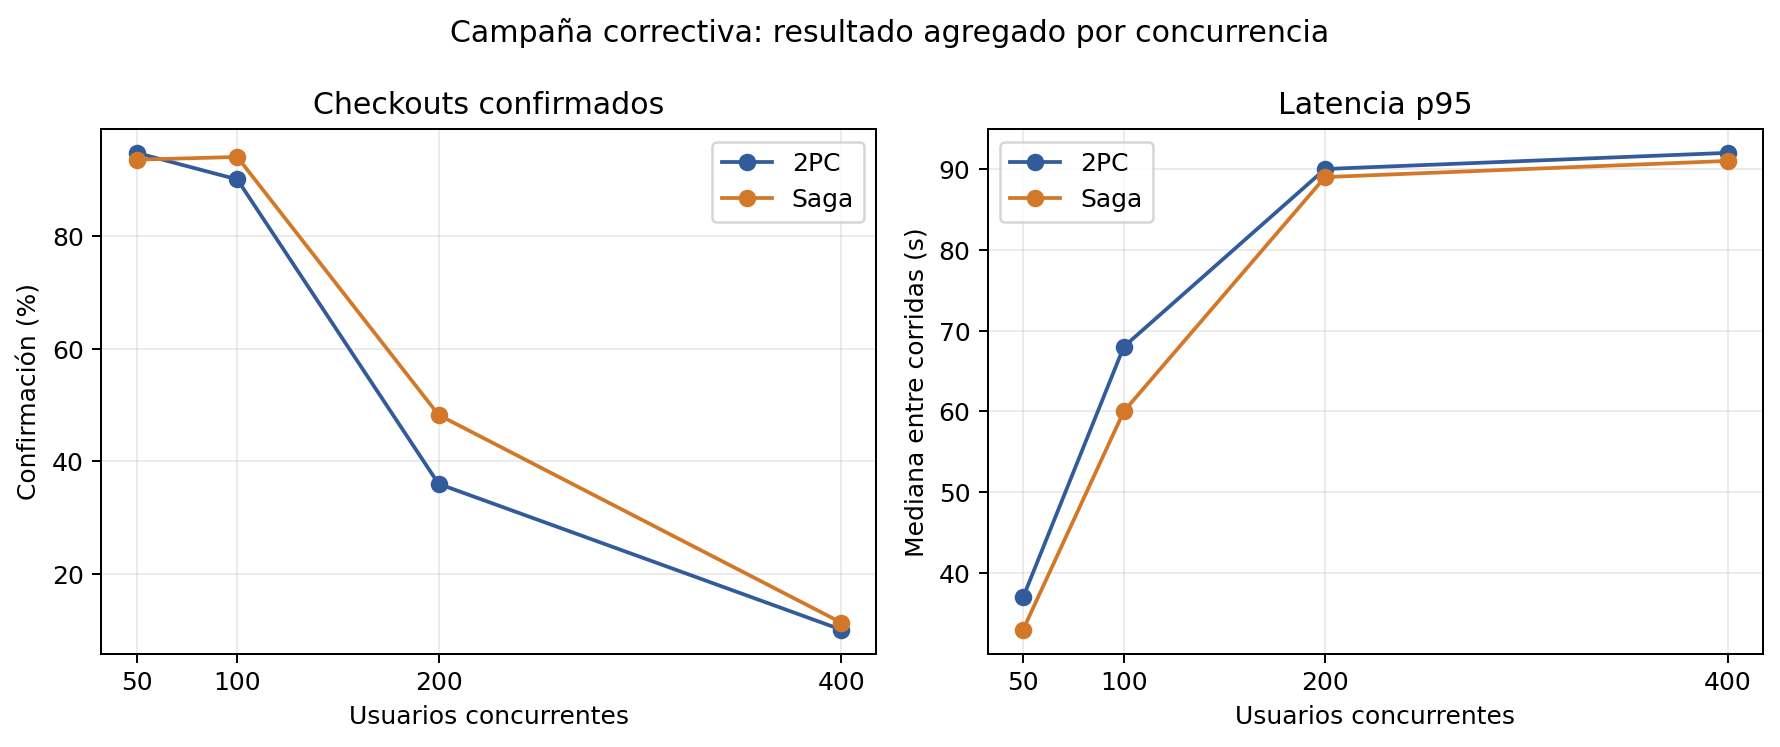
\includegraphics[width=0.96\textwidth]{../../experiments/paso8/resultados-reales/correctiva-20260905-final-v2/analisis/campana-correctiva-resumen.png}
\caption{Tasa de confirmación y mediana de p95 entre las quince corridas de cada estrategia y concurrencia. Fuente: CSV correctivo derivado sin alterar los datos crudos.}\label{fig:correctiva-resumen}
\end{figure}

En las doce comparaciones condicionadas, la mediana p95 de Saga es menor en diez, igual en una y mayor en una. Los valores exactos por permutación están entre 0,015873 y 1; ninguno cruza el umbral Bonferroni 0,004167. La figura \ref{fig:correctiva-resumen} permite describir una ventaja observada de Saga en confirmación a carga media y p95 en la mayoría de condiciones, sin afirmar superioridad poblacional. Los archivos \path{comparacion_estrategias.csv}, \path{resumen_coord_concurrencia.csv} y \path{resumen_comparativo.json} conservan el cálculo completo.

\subsection{Paralelismo y motor de datos}
La desaceleración de T1 al añadir ejecutores es compatible con sobrecostes y entrada poco paralela. Es una interpretación, no un perfil causal exhaustivo. La variante JDBC particionada cambia el acceso y muestra un patrón diferente, pero no supera automáticamente el tiempo de Pandas. Para este tamaño y entorno, la complejidad operativa de Spark no se justifica por una mejora de T1 observada.

Aplicar Amdahl como ajuste mecánico produciría una fracción no escalable superior a uno para la serie sin partición. Eso no significa que exista más de un cien por ciento de trabajo serial: el modelo omite sobrecostes dependientes del número de ejecutores. Gustafson plantea otra pregunta para cargas crecientes \cite{gustafson1988reevaluating}; no corrige retrospectivamente el resultado de carga fija.

La caída de un nodo mostró un pico de latencia con resultado conservado. Es evidencia puntual de continuidad del clúster en ese escenario, no disponibilidad sostenida. El ensayo comparte anfitrión y no cubre partición prolongada ni corrupción. Los planes con tiempos menores en clúster tampoco aíslan por sí solos diferencias de caché, índices y recursos.

\subsection{Decisiones de cierre}
El cierre mantiene arquitectura y evidencias existentes, y registra deuda en lugar de modificar apresuradamente el producto. Las prioridades son idempotencia y validación de contratos, luego pruebas de recuperación y una medición oficial con recursos y tráfico definidos. La revisión bibliográfica se corrigió porque un DOI existente puede apuntar a un trabajo distinto: comprobar que el enlace abre no basta; debe coincidir con título y autores.

El producto posee instrumentos de calidad y observabilidad antes ausentes. Sin embargo, instalar Prometheus o aprobar CI no acredita un objetivo operacional. La memoria distingue esas capas para que el lector pueda reconocer el avance sin asumir garantías todavía no medidas.

\seccion{Amenazas a la validez}
La descripción histórica del candado se refiere al banco SQLite original. El piloto posterior de la sección \ref{sec:actualizacion-evidencias} elimina el candado de Python y detecta una discordancia de stock. La evaluación distribuida correctiva ejecutó 120 corridas contra microservicios y CockroachDB y ya no presenta escasez de confirmaciones; sus límites vigentes son el anfitrión compartido, el orden fijo, la saturación a 200--400 usuarios y la ausencia de historiales persistentes por operación.
\subsection{Validez interna}
\textbf{Contención del anfitrión.} Todas las ejecuciones comparten máquina y pueden sufrir carga externa. Mitigación: conservar repeticiones y recursos, aislar futuras corridas y aleatorizar orden. No se supone aislamiento retroactivo.

\textbf{Candado global y serialización.} La versión vigente de \path{experiments/paso7/coordination_lab.py} ya no crea \texttt{self.db\_lock}; el piloto conserva el escritor único de SQLite y queda como demostración local. La evidencia principal es \path{experiments/paso8/resultados-reales/correctiva-20260905-final-v2/}, ejecutada mediante Gateway, Pedidos, Ventas, Inventario y CockroachDB. Sus 30275 confirmaciones permiten analizar el flujo real, aunque no sustituyen un oráculo persistente de invariantes.

\textbf{Semillas y orden.} El cálculo de semillas varía entre estrategias y las condiciones se recorren en orden fijo. Mitigación: utilizar listas idénticas de operaciones/fallos y orden aleatorio balanceado en una réplica. Las comparaciones actuales son no emparejadas.

\textbf{Configuración y preparación.} La campaña correctiva registra cinco segundos de demora, sesenta de calentamiento y trescientos de medición en las 120 filas. Los pilotos y la rampa reducen el riesgo de comenzar con un flujo basal roto. Permanece el riesgo de cambios térmicos y carga externa durante 22,54 horas en un solo anfitrión.

\textbf{Saturación a carga alta.} La tasa de confirmación agregada cae de 94,1\,\% con 50 usuarios a 10,8\,\% con 400. Esta caída es un resultado del entorno y no invalida las corridas, pero limita la estimación de latencia del trabajo completado porque aumenta la censura por timeout. Se reportan confirmaciones y fallos junto con cada percentil.

\subsection{Validez externa}
\textbf{Carga sintética.} Los 400 compradores y 29 productos redistribuidos reducen la concentración artificial previa, pero no representan navegación, usuarios heterogéneos ni demanda real. El alcance se limita al flujo sintético de checkout.

\textbf{Topología y pasarela.} Un anfitrión y una función de pago no modelan latencia geográfica ni fallos bancarios. Mitigación: ensayar red y participantes independientes sin usar credenciales ni pagos reales; no extrapolar los percentiles a producción.

\textbf{Catálogo artificial.} Casos generados por reglas próximas al evaluador favorecen resultados perfectos. Mitigación: etiquetas independientes, conjunto reservado y llamadas al asistente real antes de evaluar reglas frente a RAG.

\subsection{Validez de constructo}
\textbf{Inconsistencia sin exposición al fenómeno.} Las 120 tasas iguales a cero describen las comprobaciones del oráculo al terminar las corridas serializadas. No constituyen una medición válida de inconsistencia ante escrituras concurrentes independientes: el banco excluye precisamente esa fuente de anomalías. Tampoco observa todos los estados intermedios de la Saga. No se interpreta el cero como riesgo nulo ni como equivalencia de garantías entre protocolos. La réplica deberá registrar historiales y estados parciales, permitir intercalaciones reales y comprobar mediante controles positivos que el oráculo detecta las violaciones buscadas.

\textbf{Latencia mal rotulada.} Una columna de pago mide compra completa. Mitigación aplicada: nombrarla latencia de compra en el informe y conservar el nombre original en datos para trazabilidad.

\textbf{Oráculo incompleto.} El saldo neto no demuestra unicidad ni recuperación de todos los estados pendientes. Mitigación: declarar el alcance, usar historiales completos y pruebas que muten intencionalmente cada invariante.

\textbf{Recursos parciales.} CPU en segundos y memoria Python no equivalen a porcentaje CPU/RSS. Mitigación aplicada: unidades explícitas; futura instrumentación a nivel de proceso o contenedor.

\subsection{Validez de conclusión}
\textbf{Resolución de la prueba y potencia.} Con cinco observaciones por grupo, sin empates, existen \(\binom{10}{5}=252\) asignaciones de rangos bajo la hipótesis nula. El menor valor p bilateral exacto de Mann--Whitney es
\begin{equation}
p_{\min}=\frac{2}{\binom{10}{5}}=0{,}0079365\ldots
\quad > \quad
\alpha_{\mathrm{Bonferroni}}=\frac{0{,}05}{12}=0{,}0041667\ldots .
\label{eq:limite-mann-whitney}
\end{equation}
La campaña correctiva conserva cinco observaciones por grupo y presenta empates en varios p95. La prueba exacta por permutación incorpora esos empates; sus doce valores p van de 0,015873 a 1 y ninguno cruza Bonferroni. La limitación sigue siendo estructural: con cinco repeticiones no puede obtenerse una conclusión confirmatoria para una familia de doce contrastes. Una réplica futura debe aumentar repeticiones o predefinir una familia menor según la pregunta científica.

\textbf{Tamaño de efecto heterogéneo.} Para p95, \(\widehat A_{12}\) de 2PC frente a Saga varía entre 0,48 y 0,98: el solapamiento cambia por fallo y concurrencia. Esa heterogeneidad descarta trasladar al sistema real la separación perfecta del piloto SQLite y exige interpretar cada condición por separado.

La suma de violaciones no es necesariamente binomial y un cero observado no prueba riesgo nulo. Mitigación: definir una variable binaria por operación para cada invariante y reportar su intervalo por separado. Los ensayos puntuales del clúster tampoco permiten inferir disponibilidad sostenida; se mantienen como observaciones descriptivas.

\seccion{Calidad del producto}
\subsection{Modelo y criterios}
ISO/IEC 25010:2023 organiza nueve características de calidad del producto; ISO/IEC 25023:2016 aporta medidas \cite{iso25010_2023,iso25023_2016}. Las normas no imponen los umbrales académicos de cobertura o complejidad usados aquí. Esos objetivos proceden de la guía y deben interpretarse según alcance y método.

La tabla \ref{tab:iso} distingue evidencia favorable, parcial y ausente. No se declara certificación ISO ni conformidad integral por disponer de un CSV. La seguridad requiere pruebas y configuración coherentes, mientras que la mantenibilidad requiere que el código sea comprensible además de superar un umbral.

\begin{table}[H]\centering\small
\caption{Evaluación por características ISO/IEC 25010:2023.}\label{tab:iso}
\begin{tabularx}{\textwidth}{lX}
\toprule Característica & Evidencia y límite\\\midrule
Adecuación funcional & Flujos y pruebas implementados; no aceptación completa de todos los recorridos.\\
Eficiencia & Carga oficial de 50 usuarios/60 s: P95 agregado 610 ms; no cumple el umbral de 500 ms. Una sola corrida no permite estimar un IC95 del P95.\\
Compatibilidad & Contratos HTTP/gRPC; Pact y ensayo completo entre consumidores no acreditados.\\
Capacidad de interacción & Interfaces web/Android; sin estudio formal de usuarios.\\
Fiabilidad & Ventana oficial de 3600 s: 3588/3588 sondeos, 100\,\% (IC95\,\% Wilson 99{,}8931--100\,\%); en carga, 0/2112 respuestas 5xx (límite superior 0{,}1816\,\%).\\
Seguridad & JWT, restricciones de exposición y pruebas negativas; no auditoría integral.\\
Mantenibilidad & Cobertura instrumentada 82{,}31\,\% y PMD máximo 9; cumplimiento acotado porque varios módulos conservan filtros estrechos de JaCoCo.\\
Flexibilidad & Contenedores y configuración; no ensayo multientorno exhaustivo.\\
Seguridad operacional & Riesgos de stock/pago identificados; no análisis completo de daño operacional.\\\bottomrule
\end{tabularx}
\end{table}

\subsection{Cobertura y complejidad}
La tabla \ref{tab:cobertura} procede de los informes de cobertura y sus notas de alcance. Las líneas corresponden a clases instrumentadas, en particular lógica de negocio; no incluyen necesariamente controladores, infraestructura, entidades, SPA o código generado. Un 100\,\% de ocho líneas no prueba todo el servicio.

\begin{table}[H]\centering\small
\caption{Cobertura en el alcance de los informes disponibles.}\label{tab:cobertura}
\begin{tabular}{lrrr}
\toprule Módulo & Cubiertas & Medidas & Porcentaje\\\midrule
Inventario & 8 & 8 & 100,00\\
Órdenes a proveedores & 47 & 51 & 92,16\\
Pedidos & 104 & 129 & 80,62\\
Productos & 23 & 23 & 100,00\\
Usuarios & 321 & 358 & 89,66\\
Ventas & 27 & 27 & 100,00\\
armado-ia & 405 & 540 & 75,00\\\bottomrule
\end{tabular}
\end{table}

El umbral del 70\,\% se verifica directamente desde los siete XML mediante \evidencia{docs/evidencias/cobertura/verificar_umbral.py}{\texttt{verificar\_umbral.py}}. El resultado versionado \path{informe-umbral-70.json} confirma siete de siete módulos aprobados; el mínimo es 75,00\,\% en \texttt{armado-ia}. La comprobación no depende de una publicación externa en Codecov y conserva el alcance parcial de las clases instrumentadas.

El informe específico reciente de \evidencia{docs/experimentos/resultados/iso25010/complejidad/summary.csv}{complejidad} registra máximos por método de 7 en gateway, 8 en inventario, 9 en órdenes a proveedores, 7 en pedidos, 8 en productos, 9 en usuarios y 7 en ventas. Sustituye en esta memoria la afirmación antigua de máximo 20, que aún aparece en resúmenes anteriores. Los siete valores son inferiores a diez; no se extiende esa medición PMD al servicio Python.

\subsection{CI, carga y observabilidad}
Se verificó la demostración rojo/verde de GitHub Actions mediante dos ejecuciones concretas de \emph{CI-CD quality gate}: la \href{https://github.com/JoseLozanoMorales/TiendaTech/actions/runs/33554959074}{ejecución roja} concluyó en \texttt{failure} sobre el commit \texttt{f58869b}, mientras que la \href{https://github.com/JoseLozanoMorales/TiendaTech/actions/runs/33557738789}{ejecución verde} concluyó en \texttt{success} sobre \texttt{bd027f0}. Ambas fueron disparadas por \texttt{pull\_request}; los PR \#81, \#82 y \#83 conservan la secuencia de fallo intencional, reversión y corrección final. Son ejecuciones de CI, no solicitudes de incorporación de cambios. La publicación de imágenes en Docker Hub pertenece a otro workflow y se activa después de que el quality gate de \texttt{main} finaliza satisfactoriamente.

El registro \path{docs/evidencias/paso9-ci-rojo-verde.md} concilia cada enlace con su resultado, evento y commit mediante la API de GitHub. También documenta el BOM UTF-8 introducido durante la reversión y su corrección, de modo que el fallo rojo queda separado de ese efecto colateral de compilación. Con esta evidencia versionada, C7 deja de figurar como deuda documental en la tabla \ref{tab:deuda}; la verificación no implica que futuras ejecuciones o publicaciones queden aprobadas automáticamente.

La prueba de carga previa registró 1911 solicitudes y 862 fallos. El diagnóstico relacionaba parte del problema con respuestas de productos y con limitación de solicitudes por IP; no constituía aprobación de rendimiento. Una repetición posterior de la misma prueba oficial de \texttt{tests/load/} (50 usuarios, rampa 5/s, 60s), documentada con sus métricas crudas en \href{https://github.com/JoseLozanoMorales/TiendaTech/blob/b690470163513c757dd51cb8d47677d09955fda8/docs/evidencias/paso10-item5-grafana-carga.md}{carga y panel Grafana}, registró 2194 solicitudes y 1894 fallos (86,3\,\%). Se confirmó la causa en el código real de \texttt{GatewayTrafficFilter.java} (líneas 41--64): el límite de 300 solicitudes por 60\,s por IP de origen, activado porque el generador de carga corre desde un único host y por tanto un único par de transporte. Los \texttt{.csv} adjuntos confirman que el 100\,\% de los fallos son \texttt{429}; ninguno es \texttt{5xx}. Sigue sin haber una prueba de carga distribuida desde múltiples orígenes que evalúe el sistema sin ese límite por IP.

El repositorio contiene métricas Prometheus, logs JSON, recolección Alloy y configuración de Grafana. La actualización del 4 de septiembre aporta evidencia operativa puntual: se agregó un Grafana local (\texttt{docker-compose.yml}) cuyo datasource y dashboard se cargan por provisioning como código (\texttt{ops/observability/grafana/provisioning/}), no por importación manual, y se capturó con datos reales de la repetición de carga anterior (\href{https://github.com/JoseLozanoMorales/TiendaTech/blob/b690470163513c757dd51cb8d47677d09955fda8/docs/evidencias/paso10-item5-grafana-carga.md}{captura del panel}). Se aportan además trazas OpenTelemetry separadas de checkout y de incorporación al carrito, con un identificador por operación, incluyendo el canal TCP crudo entre \texttt{pedidos-service} e \texttt{inventario-service}, que por transportar JSON sobre un \texttt{Socket} plano en vez de HTTP quedaba fuera del alcance de la auto-instrumentación y no aparecía en ninguna traza; se instrumentó manualmente con spans \texttt{reservation.tcp.reconcile} y propagación del \texttt{traceparent} dentro del propio mensaje (\href{https://github.com/JoseLozanoMorales/TiendaTech/blob/b690470163513c757dd51cb8d47677d09955fda8/docs/evidencias/paso10-item6-trace-distribuida.md}{traza distribuida completa}). La disponibilidad de una hora y la tasa de errores 5xx de la corrida oficial ya se midieron (100\,\% de disponibilidad sobre 3600\,s continuos frente al objetivo de 99,5\,\%, y 0\,\% de respuestas 5xx sobre 2112 solicitudes): ambas cumplen. Permanece sin medir el p95 productivo bajo múltiples orígenes de carga simultáneos; tampoco se infiere cobertura E2E o de la SPA a partir de pruebas unitarias Java.

La sesión posterior del 4 de septiembre conserva una repetición estable en \href{https://github.com/JoseLozanoMorales/TiendaTech/blob/b690470163513c757dd51cb8d47677d09955fda8/docs/experimentos/resultados/iso25010/2026-09-04T08-44-12/ejecucion.md}{el registro de ejecución ISO}: 2112 solicitudes, cero fallos, 36,45 solicitudes/s y p95 agregado de 610 ms, contrastados con el CSV de \texttt{load-final/}. El p95 no alcanza el objetivo menor a 500 ms; cero fallos observados no garantiza fiabilidad general. La disponibilidad de una hora concluyó después de 3600\,s con 3588 de 3588 muestras exitosas: 100\,\% frente al objetivo de 99,5\,\%. Esta sesión ISO y la campaña correctiva responden preguntas distintas y no mezclan sus resultados.


Las figuras \ref{fig:grafana-carga} y \ref{fig:jaeger-compra} hacen visible la evidencia operativa descrita: la primera corresponde al panel capturado durante la carga conjunta y la segunda a las trazas exportadas en esa sesión. Son fotografías de una ejecución fechada; las métricas crudas y los JSON exportados siguen siendo la fuente auditable.

\begin{figure}[H]\centering
\includegraphics[width=0.95\textwidth]{../../release/screenshots/grafana-carga-conjunta.png}
\caption{Dashboard Grafana con datos reales durante la sesión conjunta de carga. Fuente: evidencia propia del Paso 10.}\label{fig:grafana-carga}
\end{figure}

\begin{figure}[H]\centering
\includegraphics[width=0.95\textwidth]{../../release/screenshots/jaeger-traza-compra.png}
\caption{Trazas distribuidas exportadas durante la sesión conjunta; incluyen el recorrido instrumentado y el canal TCP. Fuente: evidencia propia del Paso 10.}\label{fig:jaeger-compra}
\end{figure}

\seccion{Gestión de la revisión cruzada}
\subsection{Criterio de respuesta}
La tabla \ref{tab:issues} recoge las incidencias 16--78 recuperadas en el corte: 63 registros, de los cuales 53 figuran cerrados y 10 abiertos. Los issues 40, 46 y 48 fueron contrastados con 41, 47 y 49, recibieron una respuesta con evidencia y se cerraron administrativamente como duplicados el 4 de septiembre de 2026. Los diez abiertos restantes corresponden al trabajo pendiente identificado en el proyecto actual.

AC significa aceptar y corregir según la respuesta publicada; AD significa aceptar y diferir en este cierre documental; R significa rebatir con justificación. El estado de GitHub y la acción documental son columnas distintas. Las respuestas enlazadas contienen la justificación y, cuando existen, referencias a commits. Un cierre administrativo no constituye por sí solo prueba de ejecución ni invalida los límites de las secciones de calidad y método.

Los abiertos con corrección parcial o pendiente se incorporan como deuda explícita; AD no significa que se haya alterado el proyecto. El registro de los tres duplicados se conserva para evitar contar dos veces una misma corrección, aunque su consolidación administrativa ya quedó realizada.


{\small\begin{longtable}{p{0.6cm}p{6.8cm}p{1.7cm}p{1.1cm}p{2.8cm}}
\caption{Respuesta y evidencia individual de revisión cruzada.}\label{tab:issues}\\
\toprule N.º & Observación & Estado & Acción & Evidencia\\\midrule\endfirsthead
\toprule N.º & Observación & Estado & Acción & Evidencia\\\midrule\endhead
16 & Aplicar framework para el frontend & Cerrado & AC & \href{https://github.com/JoseLozanoMorales/TiendaTech/issues/16#issuecomment-5499536102}{Respuesta 16} \\
17 & Aplicar temas de tareas formativas al proyecto & Cerrado & AC & \href{https://github.com/JoseLozanoMorales/TiendaTech/issues/17#issuecomment-5499878376}{Respuesta 17} \\
18 & Investigación de temas de la materia aplicables al proyecto & Cerrado & AC & \href{https://github.com/JoseLozanoMorales/TiendaTech/issues/18#issuecomment-5499810621}{Respuesta 18} \\
19 & Hacer que usuarios no dañe todo el proyecto & Cerrado & AC & \href{https://github.com/JoseLozanoMorales/TiendaTech/issues/19#issuecomment-5499881456}{Respuesta 19} \\
20 & Primera versión de aplicación móvil & Cerrado & AC & \href{https://github.com/JoseLozanoMorales/TiendaTech/issues/20#issuecomment-5499700698}{Respuesta 20} \\
21 & Primera versión de la IA asistente & Cerrado & AC & \href{https://github.com/JoseLozanoMorales/TiendaTech/issues/21#issuecomment-5499702639}{Respuesta 21} \\
22 & Aplicación móvil finalizada & Cerrado & AC & \href{https://github.com/JoseLozanoMorales/TiendaTech/issues/22#issuecomment-5499884436}{Respuesta 22} \\
23 & Asistente de IA finalizado & Cerrado & AC & \href{https://github.com/JoseLozanoMorales/TiendaTech/issues/23#issuecomment-5499887488}{Respuesta 23} \\
24 & Arreglar estructura del proyecto & Cerrado & AC & \href{https://github.com/JoseLozanoMorales/TiendaTech/issues/24#issuecomment-5499806741}{Respuesta 24} \\
25 & Implementar validación JWT en el API Gateway & Cerrado & AC & \href{https://github.com/JoseLozanoMorales/TiendaTech/issues/25#issuecomment-5499444070}{Respuesta 25} \\
26 & Configurar JWT\_SECRET compartido entre Gateway y usuarios-service & Cerrado & AC & \href{https://github.com/JoseLozanoMorales/TiendaTech/issues/26#issuecomment-5499490631}{Respuesta 26} \\
27 & Definir rutas públicas del API Gateway & Cerrado & AC & \href{https://github.com/JoseLozanoMorales/TiendaTech/issues/27#issuecomment-5499481993}{Respuesta 27} \\
28 & Crear patrón reutilizable de validación JWT & Cerrado & AC & \href{https://github.com/JoseLozanoMorales/TiendaTech/issues/28#issuecomment-5499483824}{Respuesta 28} \\
29 & Cerrar exposición pública de los puertos 8081--8086 & Cerrado & AC & \href{https://github.com/JoseLozanoMorales/TiendaTech/issues/29#issuecomment-5499486242}{Respuesta 29} \\
30 & Agregar healthcheck a usuarios-service & Cerrado & AC & \href{https://github.com/JoseLozanoMorales/TiendaTech/issues/30#issuecomment-5499570043}{Respuesta 30} \\
31 & Consolidar manejadores globales de excepciones de usuarios-service & Cerrado & AC & \href{https://github.com/JoseLozanoMorales/TiendaTech/issues/31#issuecomment-5499572163}{Respuesta 31} \\
32 & Unificar rutas de creación de usuarios & Cerrado & AC & \href{https://github.com/JoseLozanoMorales/TiendaTech/issues/32#issuecomment-5499574333}{Respuesta 32} \\
33 & Corregir respuesta HTTP al crear usuarios & Cerrado & AC & \href{https://github.com/JoseLozanoMorales/TiendaTech/issues/33#issuecomment-5499576455}{Respuesta 33} \\
34 & Documentar política común de autenticación y autorización & Cerrado & AC & \href{https://github.com/JoseLozanoMorales/TiendaTech/issues/34#issuecomment-5499578395}{Respuesta 34} \\
35 & Verificar integraciones internas con protección JWT & Cerrado & AC & \href{https://github.com/JoseLozanoMorales/TiendaTech/issues/35#issuecomment-5499580121}{Respuesta 35} \\
36 & Incorporar validación JWT en ventas-service y añadir healthcheck & Cerrado & AC & \href{https://github.com/JoseLozanoMorales/TiendaTech/issues/36#issuecomment-5499544030}{Respuesta 36} \\
37 & Configurar timeouts explícitos en InventarioClient & Cerrado & AC & \href{https://github.com/JoseLozanoMorales/TiendaTech/issues/37#issuecomment-5499542065}{Respuesta 37} \\
38 & Implementar el patrón outbox al generar una factura & Cerrado & AC & \href{https://github.com/JoseLozanoMorales/TiendaTech/issues/38#issuecomment-5499545660}{Respuesta 38} \\
39 & Guardar la factura y el evento outbox dentro de la misma transacción de base de datos & Cerrado & AC & \href{https://github.com/JoseLozanoMorales/TiendaTech/issues/39#issuecomment-5499547112}{Respuesta 39} \\
40 & Crear el proceso que reintente eventos pendientes y marque un evento como procesado solo después de la confirmación de inventario & Cerrado & AC & \href{https://github.com/JoseLozanoMorales/TiendaTech/issues/40\#issuecomment-5548128749}{Respuesta 40} \\
41 & Crear el proceso que reintente eventos pendientes y marque un evento como procesado solo después de la confirmación de inventario & Cerrado & AC & \href{https://github.com/JoseLozanoMorales/TiendaTech/issues/41#issuecomment-5499549164}{Respuesta 41} \\
42 & Añadir Circuit Breaker y reintentos seguros alrededor de la comunicación con inventario & Cerrado & AC & \href{https://github.com/JoseLozanoMorales/TiendaTech/issues/42#issuecomment-5499562481}{Respuesta 42} \\
43 & Coordinar con José la idempotencia del descuento de existencias & Abierto & AD & \href{https://github.com/JoseLozanoMorales/TiendaTech/issues/43#issuecomment-5499955308}{Respuesta 43} \\
44 & Reemplazar Map String,Integer  por GenerarFacturaRequest y aplicar @Valid. & Cerrado & AC & \href{https://github.com/JoseLozanoMorales/TiendaTech/issues/44#issuecomment-5499551129}{Respuesta 44} \\
45 & Crear DTO de salida para facturas y dejar de exponer directamente la entidad JPA & Cerrado & AC & \href{https://github.com/JoseLozanoMorales/TiendaTech/issues/45#issuecomment-5499553220}{Respuesta 45} \\
46 & Incorporar validación JWT en ordenes-proveedores-service. y añadir healthcheck & Cerrado & AC & \href{https://github.com/JoseLozanoMorales/TiendaTech/issues/46\#issuecomment-5548128977}{Respuesta 46} \\
47 & Incorporar validación JWT en ordenes-proveedores-service y añadir healthcheck & Cerrado & AC & \href{https://github.com/JoseLozanoMorales/TiendaTech/issues/47#issuecomment-5499564428}{Respuesta 47} \\
48 & Configurar timeouts explícitos en InventarioClient & Cerrado & AC & \href{https://github.com/JoseLozanoMorales/TiendaTech/issues/48\#issuecomment-5548129164}{Respuesta 48} \\
49 & Configurar timeouts explícitos en InventarioClient & Cerrado & AC & \href{https://github.com/JoseLozanoMorales/TiendaTech/issues/49#issuecomment-5499565384}{Respuesta 49} \\
50 & Añadir Circuit Breaker y reintentos seguros para la comunicación con inventario & Cerrado & AC & \href{https://github.com/JoseLozanoMorales/TiendaTech/issues/50#issuecomment-5499566316}{Respuesta 50} \\
51 & Crear OrdenCompraResponseDTO y ProveedorResponseDTO & Cerrado & AC & \href{https://github.com/JoseLozanoMorales/TiendaTech/issues/51#issuecomment-5499567221}{Respuesta 51} \\
52 & Verificar que las transiciones enviar y cancelar sean idempotentes o rechacen correctamente las repeticiones & Cerrado & AC & \href{https://github.com/JoseLozanoMorales/TiendaTech/issues/52#issuecomment-5499568157}{Respuesta 52} \\
53 & Si se aprueba gRPC: implementar el cliente suscriptor de alertas de inventario y evitar órdenes duplicadas ante reconexiones o mensajes repetidos & Abierto & AD & \href{https://github.com/JoseLozanoMorales/TiendaTech/issues/53#issuecomment-5499957575}{Respuesta 53} \\
54 & Documentar por qué /enviar y /cancelar representan transiciones de negocio en lugar de un PATCH genérico & Cerrado & AC & \href{https://github.com/JoseLozanoMorales/TiendaTech/issues/54#issuecomment-5499890678}{Respuesta 54} \\
55 & Incorporar validación JWT en pedidos-service & Cerrado & AC & \href{https://github.com/JoseLozanoMorales/TiendaTech/issues/55#issuecomment-5499893613}{Respuesta 55} \\
56 & Reutilizar OrdenCompraService como punto único de lógica al recibir alertas & Abierto & AD & \href{https://github.com/JoseLozanoMorales/TiendaTech/issues/56#issuecomment-5499959748}{Respuesta 56} \\
57 & Añadir healthcheck & Cerrado & AC & \href{https://github.com/JoseLozanoMorales/TiendaTech/issues/57#issuecomment-5499896900}{Respuesta 57} \\
58 & Configurar connect timeout y read timeout en FacturaClient, ProductoClient y UsuarioClient & Cerrado & AC & \href{https://github.com/JoseLozanoMorales/TiendaTech/issues/58#issuecomment-5499900322}{Respuesta 58} \\
59 & Crear un ApiExceptionHandler global para respuestas de error uniformes & Cerrado & AC & \href{https://github.com/JoseLozanoMorales/TiendaTech/issues/59#issuecomment-5499903875}{Respuesta 59} \\
60 & Verificar que cualquier reintento de una operación de escritura sea idempotente o utilice una clave contra duplicados & Cerrado & AC & \href{https://github.com/JoseLozanoMorales/TiendaTech/issues/60#issuecomment-5499907106}{Respuesta 60} \\
61 & Añadir Circuit Breaker y reintentos controlados en los clientes internos donde sean seguros & Cerrado & AC & \href{https://github.com/JoseLozanoMorales/TiendaTech/issues/61#issuecomment-5499917467}{Respuesta 61} \\
62 & Cambiar operaciones void por respuestas HTTP explícitas, normalmente 204 No Content & Cerrado & AC & \href{https://github.com/JoseLozanoMorales/TiendaTech/issues/62#issuecomment-5499921148}{Respuesta 62} \\
63 & Corregir códigos HTTP de creación & Cerrado & AC & \href{https://github.com/JoseLozanoMorales/TiendaTech/issues/63#issuecomment-5499923933}{Respuesta 63} \\
64 & Reemplazar mapas y entidades expuestas por DTO & Abierto & AD & \href{https://github.com/JoseLozanoMorales/TiendaTech/issues/64#issuecomment-5499962026}{Respuesta 64} \\
65 & Añadir un estado formal del pedido solo si se implementará seguimiento en tiempo real & Cerrado & R & \href{https://github.com/JoseLozanoMorales/TiendaTech/issues/65#issuecomment-5499926865}{Respuesta 65} \\
66 & Mantener TCP/WebSocket como funcionalidad separada de las correcciones urgentes & Cerrado & AC & \href{https://github.com/JoseLozanoMorales/TiendaTech/issues/66#issuecomment-5499930050}{Respuesta 66} \\
67 & Validación JWT para productos e inventario. & Cerrado & AC & \href{https://github.com/JoseLozanoMorales/TiendaTech/issues/67#issuecomment-5499814085}{Respuesta 67} \\
68 & Healthcheck para productos e inventario. & Cerrado & AC & \href{https://github.com/JoseLozanoMorales/TiendaTech/issues/68#issuecomment-5499537229}{Respuesta 68} \\
69 & Idempotencia para inventario & Cerrado & AC & \href{https://github.com/JoseLozanoMorales/TiendaTech/issues/69#issuecomment-5499933929}{Respuesta 69} \\
70 & Respuesta ante eventos repetidos & Cerrado & AC & \href{https://github.com/JoseLozanoMorales/TiendaTech/issues/70#issuecomment-5499937655}{Respuesta 70} \\
71 & Mejora de productos para respuestas incorrectas & Cerrado & AC & \href{https://github.com/JoseLozanoMorales/TiendaTech/issues/71#issuecomment-5499803326}{Respuesta 71} \\
72 & Reivisón de códigos HTTP en productos & Cerrado & AC & \href{https://github.com/JoseLozanoMorales/TiendaTech/issues/72#issuecomment-5499539698}{Respuesta 72} \\
73 & Preparación de inventario como servidor & Abierto & AD & \href{https://github.com/JoseLozanoMorales/TiendaTech/issues/73#issuecomment-5499964342}{Respuesta 73} \\
74 & Creación de contrato .proto & Abierto & AD & \href{https://github.com/JoseLozanoMorales/TiendaTech/issues/74#issuecomment-5499966747}{Respuesta 74} \\
75 & Pruebas de conexión & Abierto & AD & \href{https://github.com/JoseLozanoMorales/TiendaTech/issues/75#issuecomment-5499968939}{Respuesta 75} \\
76 & Exponer entidades & Abierto & AD & \href{https://github.com/JoseLozanoMorales/TiendaTech/issues/76#issuecomment-5499971165}{Respuesta 76} \\
77 & Revisión de rutas & Abierto & AD & \href{https://github.com/JoseLozanoMorales/TiendaTech/issues/77#issuecomment-5499973475}{Respuesta 77} \\
78 & Telemetría UDP & Abierto & AD & \href{https://github.com/JoseLozanoMorales/TiendaTech/issues/78#issuecomment-5499975479}{Respuesta 78} \\
\bottomrule\end{longtable}}
\subsection{Justificación y coste de la deuda}
La idempotencia del receptor no garantiza que ventas y proveedores propaguen una misma clave en cada reintento. Por eso el issue 43 permanece abierto aunque 69 y 70 estén cerrados. Las reservas gRPC tampoco implementan el canal de alertas solicitado por 53 y 73--75. Estos alcances distintos justifican no colapsar observaciones relacionadas como si fueran equivalentes.

La tabla \ref{tab:deuda} cubre los diez abiertos del registro \path{cierre/issues-corte.json} y los pendientes de Observaciones 2. Se separan esfuerzo de resolución y coste de arrastre: el primero estima trabajo para cerrar; el segundo describe el perjuicio mientras se posterga. No hay mediciones para monetizar ese perjuicio ni convertirlo en horas semanales. Los rangos son orientativos documentales, salvo las 8--12 h de UDP, declaradas en la respuesta al issue 78. No son horas ejecutadas ni compromisos aceptados por integrantes. Las áreas indicadas son responsables funcionales propuestos; la asignación personal corresponde al equipo.

{\footnotesize\setlength{\tabcolsep}{4pt}
\begin{longtable}{>{\raggedright\arraybackslash}p{1.7cm}>{\raggedright\arraybackslash}p{3.6cm}>{\raggedright\arraybackslash}p{4.8cm}>{\raggedright\arraybackslash}p{4.3cm}}
\caption{Deuda técnica: resolución, coste de arrastre y evidencia necesaria para cerrar.}\label{tab:deuda}\\
\toprule Origen & Pendiente y esfuerzo de resolución & Coste de arrastre mientras se difiere & Área y condición de cierre\\\midrule\endfirsthead
\toprule Origen & Pendiente y esfuerzo de resolución & Coste de arrastre mientras se difiere & Área y condición de cierre\\\midrule\endhead
43 & Clave idempotente entre clientes e inventario. 6--10 h. & Un reintento puede repetir descuentos; requiere conciliación y corrección de stock. La idempotencia del receptor aislado no protege la cadena. & Backend y pruebas: clave estable por operación y prueba de reintento sin doble movimiento.\\
53, 56, 73--75 & Alertas de stock, suscriptor, deduplicación y reconexión. 20--32 h para el grupo. & Reposición manual y posible demora ante stock bajo; implementar solo el canal sin deduplicar expone a órdenes repetidas. & Backend: contrato de alertas, servidor y cliente que delegue en OrdenCompraService; pruebas de reconexión y varios suscriptores.\\
64, 76 & DTO de entrada y salida aún parciales. 8--12 h para el grupo. & Validación dispersa, contratos ambiguos y más retrabajo al modificar clientes o servicios. & Backend y pruebas: sustituir mapas/JSON crudo por DTO validados y probar entradas inválidas.\\
77 & Rutas heredadas de productos. 3--5 h. & Documentación divergente y riesgo de romper consumidores al retirar rutas sin migración. & Backend y documentación: inventario de rutas, decisión de compatibilidad y OpenAPI concordante.\\
78 & Telemetría UDP diferida por no ser prioritaria. 8--12 h, según respuesta publicada. & Se mantiene ausente ese canal; no se ha demostrado perjuicio operacional adicional con la instrumentación HTTP actual. Reactivarlo requiere revisar contrato, red, pérdida de datagramas y operación. & Arquitectura/operaciones: la decisión y su coste quedan documentados aquí. El cierre administrativo sigue pendiente; no se afirma implementación UDP.\\
C3, C6 & La campaña correctiva aporta 30275 confirmaciones y comparación descriptiva; falta oráculo persistente por operación. & Sin historial de pagos, movimientos y compensaciones no se pueden atribuir invariantes ni validar la política CAP, aunque el flujo complete compras. & Añadir identificadores e historiales auditables, controles positivos del oráculo y partición de red controlada antes de afirmar garantías.\\
\bottomrule\end{longtable}}

Los costes de los grupos no se suman por cada issue: 53, 56 y 73--75 corresponden a una misma funcionalidad, al igual que 64 y 76. Los pendientes experimentales se relacionan con idempotencia y recuperación; se requiere planificación conjunta antes de calcular un total. No se modificaron los estados remotos de los issues durante esta revisión documental.

C2, C7, P3 y C9 se retiran de la tabla de deuda vigente porque ya cuentan con evidencia versionada: campaña con preflight, duración completa y rampa; cobertura verificable y CI rojo/verde; panel y trazas bajo carga; arranque desde volúmenes limpios; y cinco referencias específicas de coordinación. C3 y C6 permanecen por la ausencia de historiales para evaluar invariantes y CAP, no por falta de compras confirmadas.

El issue 65 se rebate porque condicionaba el estado formal al seguimiento en tiempo real, que no se acredita como implementado. Esta justificación no elimina la necesidad de estados de negocio en el laboratorio; son alcances diferentes. Los costes técnicos reales deberán reestimarse al ejecutar cada cambio y sus pruebas.

\seccion{Conclusiones}
\subsection{Respuestas a las preguntas de investigación}
\textbf{Pregunta 1: invariantes.} La respuesta sigue siendo negativa, pero cambia la causa. La campaña correctiva confirma 30275 de 49786 checkouts y elimina la insuficiencia de compras terminadas. Sin embargo, su CSV registra conteos y percentiles por corrida, no historiales persistentes suficientes para comprobar pago exacto, descuento único, stock no negativo y compensación completa por operación. La ejecución acredita concurrencia y finalización; no acredita todavía las cuatro invariantes ni la política CAP por agregado.

\textbf{Pregunta 2: rendimiento.} La campaña permite una comparación descriptiva condicionada. Saga presenta menor mediana p95 en diez de doce condiciones, empate en una y valor mayor en una; además confirma 63,4\,\% de sus checkouts frente a 58,1\,\% de 2PC en el agregado. Ninguna prueba exacta por permutación resulta significativa con Bonferroni, por lo que no se afirma superioridad poblacional. La saturación reduce la confirmación de 94,1\,\% a 50 usuarios a 10,8\,\% a 400 para ambas estrategias agregadas.

\textbf{Pregunta 3: recuperación.} La campaña ejercitó omisión y temporización y conservó miles de confirmaciones bajo ambos modos, pero los conteos finales no demuestran rollback, compensación o reanudación durable por operación. No se atribuye recuperación correcta a ninguna estrategia sin estados intermedios persistentes y un oráculo específico. El piloto local modela compensación ante una excepción de autorización, pero tampoco prueba caída y recuperación distribuida del coordinador.

\textbf{Pregunta 4: compatibilidad y RAG.} El evaluador obtuvo 120/120 aciertos, pero ejecuta reglas locales del propio banco. La respuesta es negativa respecto de validar el asistente desplegado o comparar reglas con RAG. No se dispone de respuestas de ambos enfoques sobre el mismo conjunto independiente.

\textbf{Pregunta 5: reproducibilidad distribuida.} La campaña correctiva conserva 120 filas únicas, 24 condiciones con cinco repeticiones, 60 segundos de calentamiento, 300 segundos de medición y concurrencias efectivamente alcanzadas. El preflight, los pilotos, la rampa, el CSV crudo, la validación, los resúmenes y los scripts derivados están versionados en \path{experiments/paso8/resultados-reales/correctiva-20260905-final-v2/}. Esto permite auditar estructura y cálculos; los secretos, JWT y logs detallados se excluyen deliberadamente.

\subsection{Balance acumulativo}
TiendaTech pasó de la propuesta arquitectónica a una implementación con clientes, servicios, datos distribuidos e instrumentos de prueba. La campaña correctiva muestra que el flujo basal funciona y completa decenas de miles de compras, además de cuantificar su degradación con la concurrencia. El avance es verificable, pero no elimina las incidencias abiertas ni permite convertir diferencias descriptivas sin significación corregida y sin oráculo persistente en garantías generales de una estrategia.

El análisis de Spark no mostró aceleración de T1 sin particionamiento JDBC al aumentar ejecutores. El clúster conservó una consulta durante el fallo ensayado, con un pico de latencia. Ambas conclusiones son útiles aunque no sean una confirmación de las expectativas iniciales: permiten priorizar medición y coste frente a complejidad arquitectónica.

El Paso 13 queda atendido como consolidación documental con límites explícitos. No se declara que el proyecto cumpla todos los requisitos técnicos ni que se haya obtenido aprobación de similitud, autoría o evaluación docente. La continuidad requiere resolver la deuda registrada y sustituir cada resultado parcial por evidencia del mismo alcance.

El piloto posterior de la sección \ref{sec:actualizacion-evidencias} aporta una respuesta acotada adicional a la pregunta de invariantes: el nuevo control detecta una discordancia entre inventario y movimientos en E-Saga local. Este hallazgo impide extender el cero histórico al banco corregido, pero no sustituye la campaña de comparación ni valida garantías distribuidas. Las correcciones de código y los resultados de esa futura campaña deben evaluarse por separado.

\seccion{Conclusiones individuales}
Las siguientes reflexiones conservan y actualizan los textos individuales de la memoria anterior según las evidencias del corte. Su inclusión no representa firma ni aprobación personal nueva; cada integrante mantiene la responsabilidad de revisar su texto antes de la entrega institucional.

\subsection{Jhinson Stalyn Aucatoma Celorio}
La evolución de TiendaTech me permitió comprender que una aplicación distribuida no se considera terminada únicamente porque sus servicios respondan y sus contenedores puedan levantarse. La Entrega 4 hizo visible la importancia de convertir decisiones técnicas en controles repetibles: una regla de negocio debe tener pruebas, una modificación debe atravesar un pipeline y un problema operativo debe poder observarse mediante datos. El refactor por capas fue especialmente valioso porque separó responsabilidades que antes estaban mezcladas y permitió probar la lógica sin depender de la base de datos o de otros servicios. También aprendí que la cobertura es útil como señal, pero no sustituye el diseño de casos relevantes; alcanzar el setenta por ciento tiene sentido solamente si se cubren decisiones que afectan inventario, órdenes, facturación y usuarios. La preparación de Prometheus, logs estructurados y Grafana mostró que medir un sistema requiere definir antes qué pregunta se desea responder. Finalmente, la evaluación ISO/IEC 25010 reforzó la necesidad de informar resultados honestos: una métrica pendiente debe conservarse como pendiente y no completarse con una estimación. Considero que el proyecto logró una base más mantenible y verificable, aunque todavía necesita ejecutar la observación prolongada, la carga oficial del despliegue, aunque las últimas ejecuciones de CI ya fueron verificadas. Mi principal aprendizaje es que la calidad no es una actividad final, sino una propiedad que debe incorporarse al flujo normal de desarrollo. En este cierre también reconozco que las mediciones del laboratorio no equivalen a producción: el uso de una base SQLite y un bloqueo compartido limita la comparación de estrategias. Mantener esa distinción evita atribuir garantías distribuidas a controles locales y permite orientar una siguiente iteración verificable.

\subsection{Jeremy Ruperto Gaibor Rodriguez}
Durante este proyecto confirmé que el trabajo con microservicios exige coordinar elementos que en una aplicación monolítica suelen permanecer juntos. El API Gateway, los contratos HTTP, la autenticación y la persistencia distribuida forman una cadena: un error en cualquiera de esos puntos puede afectar un flujo completo aunque cada servicio funcione por separado. Las pruebas de integración añadidas ayudan a reducir esa incertidumbre porque verifican recorridos reales hacia productos, usuarios y pedidos, mientras que las pruebas de seguridad comprueban que las rutas protegidas no queden expuestas accidentalmente. El pipeline representa otro cambio importante en la forma de trabajar. Ya no basta con que una modificación compile en la computadora de un integrante; las mismas pruebas, reglas de cobertura y construcciones deben ejecutarse en un ambiente reproducible. También comprendí el valor de hacer depender el build de los controles anteriores, pues publicar una imagen cuando existen pruebas fallidas trasladaría el riesgo hacia producción. La evaluación ISO reveló además que aprobar cobertura no implica aprobar mantenibilidad: el diagnóstico inicial de PMD encontró complejidad de 20, mientras que los informes posteriores registran máximos entre siete y nueve. Por ello, mi conclusión es que el proyecto avanzó de una demostración funcional hacia un producto con mecanismos de control, aunque su validación final depende de conservar evidencias reales, completar las mediciones operativas pendientes y mantener bajo control la complejidad después del refactor. En este cierre también reconozco que las mediciones del laboratorio no equivalen a producción: el uso de una base SQLite y un bloqueo compartido limita la comparación de estrategias. Mantener esa distinción evita atribuir garantías distribuidas a controles locales y permite orientar una siguiente iteración verificable.

\subsection{Andy Paul Sanchez Pilaloa}
El desarrollo de TiendaTech me ayudó a relacionar conceptos de arquitectura, pruebas y operación que anteriormente podía considerar independientes. La arquitectura en capas facilitó localizar la lógica de negocio y diseñar pruebas unitarias con dependencias simuladas. Esa separación también disminuye el costo de reemplazar una implementación de persistencia o comunicación, porque el dominio no necesita conocer detalles de infraestructura. La parte de observabilidad resultó igualmente significativa: un contador permite conocer la demanda, un histograma permite analizar percentiles y un gauge representa valores que suben y bajan, como las conexiones activas. Estas diferencias son esenciales para construir un dashboard que sirva para tomar decisiones y no sea solamente decorativo. La instrumentación desarrollada deja logs JSON y métricas homogéneas en siete servicios, además de Prometheus y Alloy como componentes de recolección. Sin embargo, configurar herramientas no equivale a completar la observabilidad: la correlación por trazas y la captura de Grafana con datos reales, que en un primer momento quedaron pendientes, ya se cerraron con evidencia real; la disponibilidad de una hora ya se midió después, con resultado favorable (100\,\% sobre 3600\,s continuos); permanece pendiente el p95 productivo bajo múltiples orígenes de carga. El modelo ISO/IEC 25010 y los umbrales académicos aportaron criterios para expresar esa diferencia mediante evidencia. El aprendizaje más importante fue reconocer que documentar una limitación también es una práctica profesional. Un reporte técnico útil distingue con claridad lo implementado, lo ejecutado y lo todavía pendiente, permitiendo que otra persona continúe el trabajo sin depender de afirmaciones imposibles de reproducir. Además, participar en las pruebas de seguridad, cobertura y carga me enseñó que cada resultado necesita un contexto reproducible, criterios de aceptación definidos y seguimiento de fallos antes de convertirse en una afirmación de calidad. En este cierre también reconozco que las mediciones del laboratorio no equivalen a producción: el uso de una base SQLite y un bloqueo compartido limita la comparación de estrategias. Mantener esa distinción evita atribuir garantías distribuidas a controles locales y permite orientar una siguiente iteración verificable.

\subsection{José Alejandro Lozano Morales}
La construcción acumulativa del PFC permitió observar cómo una propuesta inicial se transforma mediante decisiones arquitectónicas, implementación, validación y operación. En esta última etapa entendí que la documentación debe evolucionar junto con el código. Un diagrama, una tabla o una conclusión pierde valor cuando describe un estado anterior del repositorio; por esa razón fue necesario actualizar la evidencia de pruebas, pipeline, observabilidad e ISO/IEC 25010 sin ocultar los elementos pendientes. También considero importante la reflexión ética aplicada al proyecto. Los datos de usuarios, credenciales y tokens no pueden tratarse como simples detalles técnicos: deben protegerse, excluirse del repositorio y evitarse en logs y capturas. De igual manera, reportar una disponibilidad o latencia no medida sería una forma de desinformación, incluso si el valor pareciera razonable. La automatización reduce algunos riesgos al ejecutar pruebas y conservar reportes de manera consistente. El documento final debe funcionar como evidencia profesional y no solo como requisito académico; por eso integra los resultados favorables y las limitaciones del experimento local, junto con planes concretos de mejora. Mi conclusión personal es que un producto profesional necesita ingeniería verificable y comunicación transparente. Ambas responsabilidades pertenecen al equipo completo y deben mantenerse durante la defensa, cuando cada integrante tendrá que explicar tanto los logros como los límites reales del sistema. En este cierre también reconozco que las mediciones del laboratorio no equivalen a producción: el uso de una base SQLite y un bloqueo compartido limita la comparación de estrategias. Mantener esa distinción evita atribuir garantías distribuidas a controles locales y permite orientar una siguiente iteración verificable.


\seccion{Reflexión ética}
El Código de Ética y Práctica Profesional de Ingeniería de Software de ACM/IEEE-CS \cite{acmieee} sitúa el interés público, la calidad del producto y el juicio profesional como responsabilidades del desarrollo. En TiendaTech se traducen en decisiones concretas: no presentar pagos simulados como integración bancaria, no convertir un porcentaje de cobertura acotado en garantía de todo el sistema y no ocultar fallos para obtener una evaluación más favorable.

Las reservas y pagos tienen consecuencias potenciales para usuarios. Un reintento sin deduplicación puede descontar existencias de nuevo; una compensación incompleta puede mostrar una compra fallida con efectos persistentes. Aunque el proyecto sea académico, su documentación debe distinguir esos riesgos y explicar por qué no se recomienda usar un ensayo local como certificación productiva. Informar de un resultado negativo es una contribución técnica cuando impide una decisión basada en confianza falsa.

El manejo de credenciales y datos personales exige mínima exposición. Los secretos se suministran por configuración y no deben aparecer en commits, capturas ni logs. Antes de compartir evidencias se revisan tokens, direcciones y otros identificadores. Los datos sintéticos se rotulan como tales para evitar que se interpreten como transacciones de personas o estadísticas de un negocio real. La replicación no es una excusa para conservar innecesariamente información sensible.

La honestidad bibliográfica requiere comprobar que cada identificador corresponde a la obra citada. Reutilizar una referencia sin verificarla puede atribuir a un autor resultados que nunca publicó. Esta revisión corrigió la selección de fuentes académicas y mantuvo los estándares mediante enlaces institucionales, sin inventar DOI para cumplir una casilla formal.

El uso de IA generativa no transfiere la autoría ni la responsabilidad al asistente. Las sugerencias deben contrastarse con código y resultados; una redacción convincente puede ocultar supuestos incorrectos. Tampoco es admisible atribuir experiencias personales, firmas o aceptación a otros integrantes sin su revisión. Las reflexiones individuales se presentan para revisión y no sustituyen ese consentimiento.

Finalmente, la urgencia de entrega no justifica cambiar datos ni cerrar incidencias sin evidencia. Este informe conserva trabajo pendiente, acota estimaciones y no declara un porcentaje de similitud que no se ha medido. La obligación profesional es comunicar lo conocido y lo desconocido con suficiente claridad para que otra persona pueda evaluar el producto y continuar sin repetir errores.

\seccion{Declaraciones}
\subsection{Autoría y contribución}
El equipo AGLS está compuesto por los cuatro integrantes de la portada, con roles asignados desde la primera entrega. La tabla \ref{tab:contribuciones} resume responsabilidades y evidencia de trabajo colectivo, sin asignar porcentajes ni afirmar exclusividad sobre archivos desarrollados conjuntamente.

\begin{table}[H]\centering\small
\caption{Contribuciones por rol, sujetas a revisión final de sus autores.}\label{tab:contribuciones}
\begin{tabularx}{\textwidth}{lX}
\toprule Integrante & Contribución documentada\\\midrule
Jhinson Aucatoma & Arquitectura, ADR, modelo y distribución de datos; organización de evidencias de clúster y decisiones.\\
Jeremy Gaibor & Desarrollo e integración de servicios, comunicaciones y banco experimental; scripts y resultados incorporados al repositorio.\\
Andy Sanchez & Pruebas, cobertura, complejidad, CI, seguridad, carga e instrumentación; informes con alcance y límites.\\
José Lozano & Denominación y trazabilidad, revisión documental y de incidencias, consolidación bibliográfica y cierre acumulativo.\\\bottomrule
\end{tabularx}
\end{table}
La contribución de una persona no excluye ayuda de otra. Los commits y las respuestas de revisión constituyen evidencia de evolución, no una medición automática de esfuerzo individual. Esta memoria no añade firmas digitales ni certifica una aprobación que no haya sido comunicada.

\subsection{Uso de inteligencia artificial generativa}
Las herramientas declaradas por el documentalista para el equipo son Claude para Jhinson y Andy, y Codex para Jeremy, Andy y José. No se incorporan otras herramientas generativas por suposición. Se usaron como apoyo para análisis técnico, desarrollo, revisión y redacción, no como sustitución del trabajo ni de la responsabilidad humana. Jhinson empleó Claude en materiales de arquitectura y decisiones, cuya coherencia con los ADR y el despliegue revisó personalmente; Jeremy empleó Codex en implementación y banco de pruebas, y revisó su ejecución, código y resultados; Andy empleó Claude y Codex como apoyo en calidad, CI, seguridad, carga y revisión de su conclusión individual, y contrastó las afirmaciones con pruebas e informes; José empleó Codex en trazabilidad, revisión documental, bibliografía, tablas, figuras y LaTeX, y comprobó fuentes, rutas, compilación y presentación del PDF.

En el cierre documental, Codex asistió a José en la inspección de evidencias, conciliación de resultados, preparación de tablas y figuras, revisión bibliográfica, edición de LaTeX y comprobación del PDF; también asistió a Andy en la revisión y ampliación de su conclusión individual y en la actualización de su declaración de IA. Las secciones afectadas abarcan arquitectura, diseño del estudio, resultados, calidad, gestión de la revisión, conclusiones y declaraciones. No se atribuye un modelo, versión, prompt o procedimiento de validación más específico que el comunicado por cada integrante.

Los textos individuales requieren lectura de cada autor antes de su presentación como declaración personal. La generación asistida no demuestra ausencia de errores: las afirmaciones se mantienen vinculadas a archivos, y los resultados faltantes se declaran como no medidos. La comprobación institucional de similitud inferior al 15\,\% no se ejecutó en este cierre y no se certifica.

\subsection{Reproducibilidad documental}
La fuente principal es \path{docs/entrega4/PFC4.tex} y utiliza la bibliografía compartida \path{docs/entrega3/referenciasPFC.bib}. La compilación se realiza desde \path{docs/entrega4/} mediante pdfLaTeX, Biber y dos pasadas adicionales de pdfLaTeX, según las instrucciones del README principal. Las imágenes se resuelven con rutas relativas y los diagramas C4 se generan desde TikZ.

Para reproducir el PDF desde un clon se versionan el logo, las imágenes de \path{img/} y \path{release/screenshots/}, y las figuras derivadas. La evidencia distribuida principal conserva las 120 corridas de microservicios y CockroachDB, preflight, pilotos, rampa, resumen y validación en \path{experiments/paso8/resultados-reales/correctiva-20260905-final-v2/}. \path{analyze_corrective_comparison.py} y \path{plot_corrective_results.py} regeneran tablas y gráfica sin modificar el CSV crudo. El banco SQLite permanece como piloto histórico y no sustenta C2, C3 ni C6.

El README de esta entrega fija CPython 3.11.1, Matplotlib 3.9.0 y el identificador de la imagen TeX Live 2026; el cuaderno puede verificarse con el ejecutor estándar incluido, sin instalar Jupyter. También proporciona desde la clonación los comandos de prueba, regeneración, análisis y compilación. El 1 de septiembre de 2026, una clonación local aislada del árbol candidato completó tres pruebas, 120 corridas, el cuaderno, las figuras y la compilación de 39 páginas en 623,55 segundos (10 min 23,55 s), con 120/120 aprobaciones del oráculo y cero inconsistencias observadas. La descarga dependiente de la red se excluyó del cronómetro y el resultado no se equipara a una ejecución del sistema distribuido productivo.

El hash enlazado identifica las fuentes remotas de las mediciones. El cierre se integra en los nombres originales del documento y la bibliografía; las versiones anteriores permanecen consultables en el historial de Git.

\clearpage
\printbibliography[heading=bibnumbered,title={Bibliografía}]
\end{document}
